%%%%%%%%%%%%%%%%%%%%%%%%%%%%%%%%%%%%%%%%%%%%%%%%%%%%%%%%%%%%%%%%%%%%%%%%
%                                                                      %
%     File: Thesis_Implementation.tex                                  %
%     Tex Master: Thesis.tex                                           %
%                                                                      %
%     Author: Andre C. Marta                                           %
%     Last modified :  2 Jul 2015                                      %
%                                                                      %
%%%%%%%%%%%%%%%%%%%%%%%%%%%%%%%%%%%%%%%%%%%%%%%%%%%%%%%%%%%%%%%%%%%%%%%%

\chapter{GPU architectural characterization to decoupled V-F}
\label{chapter:gpu_char}
The first objective of this thesis is to provide a methodology to uncover the use of non-conventional voltage-frequency pairs on regularly deployed \acrshort{gpu}s to improve their energy efficiency.
This chapter introduces the developed methodology used to assess the usability and benefits of non-default voltage values on top of the traditional device frequency scaling. 

The developed methodology allows for:
\begin{itemize}
    \item The determination of which \acrshort{gpu} components establish the voltage guardband size;
    \item The identification of the architectural component responsible for the wrong application output (computational error or memory corruption);
    \item The determination of the relation between the application of non-conventional V-F scaling on both \acrshort{dvfs} domains and the resulting performance, power and energy consumption, as well as energy efficiency.
\end{itemize}

By following the workflow depicted in Figure~\ref{fig:gpu_char}, the chapter introduces a set of benchmarks that stress each individual \acrshort{gpu} \acrshort{dvfs} domain and component to find $V_{min}$ (see Section~\ref{sec:char_meth}), the frequency-dependent minimum operating voltage that (still) leads to correct GPU operation. It continues by presenting the experimental setup and testing procedure on two different \acrshort{gpu} architectures, the AMD Vega 10 Frontier Edition and AMD Radeon 5700 XT (see Section~\ref{sec:ex_setup}). The establishment of a usable voltage range across the frequency spectrum (presented in Section~\ref{sec:limiting_components}) allows for the creation a voltage-frequency exploration and usable space (top right chart of Figure~\ref{fig:gpu_char}). The chapter finishes with Section~\ref{sec:gpu_behaviour}, with an evaluation of the performance, energy consumption and Energy Delay Product (\acrshort{edp}), for the given benchmarks when subject to non-conventional V-F scaling (bottom right chart of Figure~\ref{fig:gpu_char}). 
Even though the delay of a \acrshort{cmos} circuit is inversely proportional to the supply voltage $V_{DD}$, the dynamic power is proportional to the square of $V_{DD}$ (and so, energy consumption and \acrshort{edp} will be directly proportional to $V_{DD}$), computing the \acrshort{edp} brings the additional benefit of directly analyzing the effect of voltage change in the energy efficiency of the device.

\begin{figure}[htb]
  \centering
  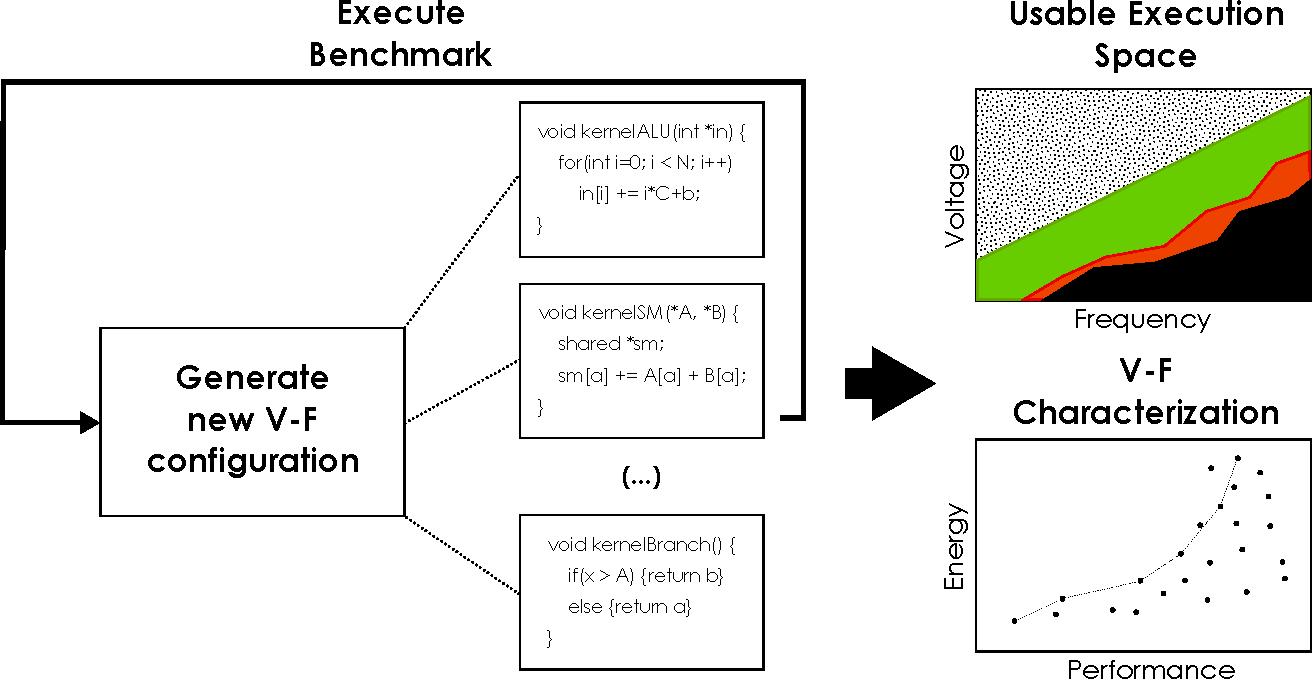
\includegraphics[width=0.8\textwidth]{Figures/GPU_characterization/gpu_char.pdf}
  \caption{Overview of the methodology and its objective outputs.}
  \label{fig:gpu_char}
\end{figure}




\section{Characterization Benchmarks}
\label{sec:char_meth}

The devised set of benchmarks,  presented in Table~\ref{tab:benchmarks} and made publicly available as open-source\footnote{https://github.com/hpc-ulisboa/nonconventional-dvfs}, individually characterize the different components of the \acrshort{gpu} architecture when subjected to the two \acrshort{dvfs} domains: \textit{core} and \textit{global memory}. The tested architectural components are \acrshort{dram}, Shared Memory, Cache L2 and \acrshort{alu}. In more detail, the memories experiments cover the reading and writing operations, as well as the prolonged effects of undervoltage on memory retention, while the \acrshort{alu} tests include the Multiply and Accumulate (MAC) and non-linear operations, as well as the impact of branches. Overall, the developed benchmarks were crafted not only with the intention of stressing the individual components, but doing so in a way that helps to answer the questions presented at the beginning of this chapter. Additionally, a coarser and more representative kernel that stresses multiple architecture elements in many \acrshort{gpgpu} applications - the reduction - is also evaluated.


\begin{table}[htb]
    \caption{Devised set of kernels to characterize GPU to Non-Conventional DVFS}
    \vspace{-5pt}
    \begin{center}
        \resizebox{\textwidth}{!}{%
        \begin{tabular}{lll}
            \hline
            \textbf{Micro-kernels}        & \textbf{Data Type} & \textbf{Objective} \\ \hline
            DRAM                                    & FP32, INT32                     & Minimum Read \& Write voltage, bit-flip, data-corruption                     \\[0.2em]
            &  & Effect of memory to compute bounded kernel on Core DVFS                     \\[0.5em]
            Cache L2                                & INT32                           & Minimum Read \& Write voltage, data-corruption                   \\[0.5em]
            Shared Memory                           & INT32                           & Minimum Read \& Write voltage, data-corruption                    \\[0.5em]
            ALU                                     & FP64/32/16, INT64/32/16/8       & Computation errors due to timing violations                   \\[0.5em]
            SFU                                     & FP64/32/16                      & Computation errors due to timing violations                   \\[0.5em]
            Branch                                  &                                 & Minimum voltage for correct schedualing operation                   \\[0.5em] %\hline
            %\textbf{App. kernels}   & \textbf{Data Type}              & \textbf{Objective} \\ \hline
            Mix (reduction)                               & FP64/32/16                      & Simultaneous impact of stressing multiple GPU components                   \\\hline
        \end{tabular}%
        }
    \end{center}
    \label{tab:benchmarks}
\end{table}

On the listed benchmarks, the placeholder \texttt{DATA\_TYPE} is used to represent the different tested data types. By following Table~\ref{tab:benchmarks}, this generic keyword is replaced by a standard integer and half, single and double precision data types, depending on the benchmark. 
The objective is to assess the effect of changing the type of operands and resulting effect on the computation precision on the critical path.


To guarantee that no compiler optimizations are performed on the tested variables, the keyword \texttt{volatile} is used.


\subsubsection{DRAM}
\label{sec:DRAMbench_exp}

The benchmark on Listing~\ref{lst:DRAMbench} was designed (and validated through \acrshort{gpu} counters) to determine the impact of V-F scaling on the \acrshort{gpu} \acrshort{dram} when executing a compute-bounded kernel.

In the presented kernel, each thread is responsible for accessing the global memory and retrieving two values. The accesses are sequential between threads to guarantee the maximum memory throughput and no accessing hazards. 
These two values are summed and placed on an output vector. The constant $C$ determines the distance between accesses, and its value is sufficiently large to guarantee that the new data to be fetched is not present on the local caches.
For each data fetch, the defined \texttt{OPS} value controls the number of arithmetic operations to be performed before the data is written back on the \acrshort{dram}. A lower \texttt{OPS} value decreases the time between memory access, resulting in a more memory intensive kernel, that depending on the global memory bandwidth and throughput, can become memory-bounded. On the other hand, a higher \texttt{OPS} value results in the memory accesses to be more spaced in time, leading to a less memory intensive kernel and, eventually, to a compute bounded kernel.

The \acrshort{dram} \acrshort{dvfs} domain is responsible for controlling the voltage and frequency of the \acrshort{gpu} global memory. This \acrshort{dvfs} domain affects the memory throughput both on the reading and writing operations. With the characterization of this \acrshort{dvfs} domain, it is possible to judge the weight of the global memory on the overall power and energy consumption and the impact of \acrshort{dram} performance when executing a more memory-bounded kernel. On the other hand, by assessing the \acrshort{gpu} performance and energy consumption, with the same kernel, while acting on the core \acrshort{dvfs} domain, it provides an understanding of how to best tune the core when the performance bottleneck is not within it.

\begin{figure}[h]
    \begin{lstlisting}[language=C, caption=DRAM Benchmark Code, label=lst:DRAMbench, basicstyle=\footnotesize\ttfamily,abovecaptionskip=0pt, captionpos=b]
    void  DRAMcode(DATA_TYPE *IN0, DATA_TYPE *IN1, DATA_TYPE *OUT) {
        const int ite = (blockIdx.x * THREADS + threadIdx.x) % MEM_BLOCK;
        volatile register DATA_TYPE r0;
        
        #pragma unroll
        for (int i = 0; i < N; i++) {
            r0= IN0[i * C + ite] + IN1[i * C + ite];
            #pragma unroll
            for(int j = 0; j < OPS; j++)  
                asm volatile ("");
            OUT[threadId] = r0;
        }
    }
    \end{lstlisting}
\end{figure}

Listing~\ref{lst:DRAMbitflip} renders a benchmark that was specifically designed to evaluate the occurrence of the phenomenon called \textit{bit-flip} and the preservation of the data in memory when exposed to undervoltage. A \textit{bit-flip} is an unintentional state switch (from 0 to 1, or vice versa) of any individual bit stored on a \acrshort{dram} or other kinds of volatile memories. The work of Kim~\cite{kim_flipping_2014} exposed the existence of \textit{bit-flipping} on \acrshort{cpu} \acrshort{dram}, induced by the continuous activation of a \acrshort{dram} row that corrupts the data in near-by rows. The work was of such significant importance that the benchmark called \textit{rowhammer}\footnote{https://github.com/google/rowhammer-test} to test this exact problem started to be of severe importance to guarantee data integraty in novel systems. The benchmark on Listing~\ref{lst:DRAMbitflip} is a GPU implementation of \textit{rowhammer} that is going to be used to assess if undervolting the GPU can increase the possibility of such problem.

\begin{figure}[h]
    \begin{lstlisting}[language=C, caption=DRAM Bit-Flip Stress Test Code - \textit{rowhammer} inspired  benchmark, label=lst:DRAMbitflip, basicstyle=\footnotesize\ttfamily,abovecaptionskip=0pt, captionpos=b]
    void  DRAMstresser(DATA_TYPE *IN, DATA_TYPE *OUT) {
        const int ite = threadIdx.x;
        volatile register DATA_TYPE r0;
        
        // Initiate output memory
        OUT[ite] = IN[ite];
        OUT[ite + THREADS * BLOCKS] = IN[ite + THREADS * BLOCKS];
        
        for (int i = 0; i < N; i++) {
            r0 = IN[ite];
            #pragma unroll
            for(int j = 0; j < OPS; j++)  
                asm volatile ("");
            OUT[ite] = r0;
        }
    }
    \end{lstlisting}
\end{figure}

For the memory tests (\acrshort{dram}, Cache and Shared Memory), only the integer data type was considered, since the effects on memory are the same for floating-point operations and it is easier to identify data corruption with integer data types.


\subsubsection{Cache}

As previously stated, even though the caches are part of the memory subsystem, they are under the \textit{core} \acrshort{dvfs} domain. The devised benchmark, presented on   Listing~\ref{lst:CacheL2bench}, follows a similar stressing pattern to Listing~\ref{lst:DRAMbench}. However, with the addition of the external \texttt{k} loop, the access pattern is repeated, and so, after the first execution, the data will be available on one of the two levels of cache. Hence, this kernel is then able to test both the state machine responsible for establishing the communication between the cache and the \acrshort{dram} and the cache itself (results verified with \acrshort{gpu} counters).

For this benchmark, the number of issued requests to the cache and to the DRAM-cache controller stays the same independently of the \texttt{OPS} value. However, the frequency of those requests is inversely proportional to \texttt{OPS}.

\begin{figure}[h]
    \begin{lstlisting}[language=C, caption=CacheL2 Benchmark Code, label=lst:CacheL2bench, basicstyle=\footnotesize\ttfamily,abovecaptionskip=0pt, captionpos=b]
    void  CacheL2code(DATA_TYPE *IN, *OUT) {
        const int ite = blockIdx * THREADS + threadIdx;
        volatile DATA_TYPE r0;
        
        for (k=0; k<N; k++) {
            #pragma unroll
            for(j=0; j<COMP_ITE; j++) {
                r0= IN[ite];
                #pragma unroll
                for(m=0; m<OPS; m++)    
                    asm volatile ("");
                OUT[ite] = r0;
            }
        }
    }
    \end{lstlisting}
\end{figure}

\subsubsection{Shared Memory}

The proposed benchmark to characterize the Shared Memory is presented in Listing~\ref{lst:SMcode}. This component is shared between threads in the same \acrshort{cu}/\acrshort{sm} and is used to ensure the communication between the different executing threads. As so, the developed benchmark uses this component to move data around. Similarly to the \acrshort{dram} and cache kernels, the \texttt{OPS} variable controls the time distance between memory requests, allowing to control the level of stress over this component and while assessing its behaviour. To guarantee a correct and repeatable execution, the synchronization directive \texttt{\_\_syncthreads()} is used to synchronize all the threads that use the same shared memory.

\begin{figure}[h]
    \begin{lstlisting}[language=C, caption=Shared Memory Benchmark code, label=lst:SMcode, basicstyle=\footnotesize\ttfamily, abovecaptionskip=0pt, captionpos=b]
    void  SharedMemorycode(DATA_TYPE *IN, DATA_TYPE *OUT) {
        __shared__ DATA_TYPE shared[THREADS];
        const int ite = blockIdx * THREADS + threadIdx;
        const int t = threadIdx.x;
        const int tr = THREADS - t - 1;
        
        volatile register DATA_TYPE r0 = IN[ite];
        
        for (int i = 0; i < N; i += UNROLL_ITE) {
            #pragma unroll
            for(int j = 0; j < UNROLL_ITE; j++)  
                shared[t] = r0;
                __syncthreads();
                for(int k = 0; k < OPS; k++) 
                    asm volatile ("");
                r0 = shared[tr];
                __syncthreads();
        }
        OUT[ite] = r0;
    }
    \end{lstlisting}
\end{figure}

\subsubsection{Arithmetic and Logic Unit (ALU)}

The arithmetic and logic unit (\acrshort{alu}) is responsible for performing all the \acrshort{gpu} computations.  Being the component that performs such a different number of operations, a set of benchmarks was devised to stress this component in different ways. Overall, the focus of testing this component was on the understanding the degree of computational errors that may occur when overly undervoltage is applied, these resulting from timing violations across the critical path. Of significant importance when investigating the timing faults on the critical path is to test the influence of data dependencies in the code, as these may influence how the warps scheduler orders the threads for execution on the \acrshort{cu}/\acrshort{sm}s. The devised benchmarks that test the \acrshort{alu} were designed to use all the available threads on the \acrshort{gpu}.

In Listing~\ref{lst:MACbench}, a greater emphasis was devoted to the \acrshort{mac} operation due to its prevalence in the Deep Learning (DL) domain. To test the influence of data  dependencies on the application, and so the way the scheduler handles the execution of the different threads, a value between $0$ and $5$ is assigned to variable \texttt{d} . When $d=0$, no dependencies exist in the code. The setup with $d=1$ represents the worst-case scenario, since it introduces Read-after-Write (RaW) dependencies between all operations. This particular dependency setup was emphasized in the presented study, due to the prevalence of such type of data dependencies in kernels executed by DL workloads. On the other hand, the setup with $d=3$ was considered a general case, where some dependencies still exist in the code, but the scheduler can mask some of them.



\begin{figure}[htpb]
    \begin{lstlisting}[language=C, caption=MAC Benchmark Code, label=lst:MACbench, basicstyle=\footnotesize\ttfamily, abovecaptionskip=0pt, captionpos=b]
    void  MACcode(DATA_TYPE *IN, DATA_TYPE *OUT) {
        const int ite = (blockIdx * THREADS + threadIdx) * 4;
        
        volatile DATA_TYPE r0, r1, r2, r3, r4, r5;
        
        r0=IN[ite];  r1=IN[ite+1];  r2=IN[ite+2]; 
        r3=IN[ite+3];  r4=IN[ite];  r5=IN[ite+1];
        
        for(j=0; j<COMP_ITE; j++) {
            r0 += r0 * r{0-d};
            r1 += r1 * r{1-d}; 
            r2 += r2 * r{2-d};
            r3 += r3 * r{3-d}; 
            r4 += r4 * r{4-d};
            r5 += r5 * r{5-d};
        }
        OUT[ite/4] = r0;
    }
    \end{lstlisting}
\end{figure}


\subsubsection{Non-Linear Operations}
    
Besides the \acrshort{mac} operation, the \acrshort{alu} also computes a set of non-linear functions, including exponential, logarithmic and trigonometric operations. For such purpose, it uses the special function unit (\acrshort{sfu}). The devised benchmark presented in Listing~\ref{lst:NonLinearbench} tests those operations to find if the undervoltage mechanism, when in use, introduces some modifications in the critical path and so, negatively influences the guardband size.
    
\begin{figure}[htpb]
    \begin{lstlisting}[language=C, caption=Non-linear Operations Benchmark Code, label=lst:NonLinearbench, basicstyle=\footnotesize\ttfamily, abovecaptionskip=0pt, captionpos=b]
    void  NonLinearcode(DATA_TYPE *IN, DATA_TYPE *OUT) {
        const int ite = (blockIdx * THREADS + threadIdx) * 4;
        
        volatile DATA_TYPE r0, r1, r2, r3;
        
        r0=IN[ite]; r1=IN[ite+1]; r2=IN[ite+2]; r3=IN[ite+3];  
        
        for(j=0; j < N; j+= UNROLL_ITE) {
            #pragma_unroll
            for(j=0; j < UNROLL_ITE; j++) {
                r0 = exp(r2);  
                r1 = cos(r3);
                r2 = log(r0);   
                r3 = sin(r1);
            }
        }
        OUT[ite/4] = r0;
    }
    \end{lstlisting}
\end{figure}

\subsubsection{Branches}

Listing~\ref{lst:Branchesbench} renders the devised benchmark to tests the influence on the execution of branches on a kernel. \acrshort{simt} processors do not favor the existence of branches on code, since it prevents the simultaneous execution of all threads. 
The scheduler's job is to organize the running threads in wavefronts to be simultaneously executed depending on the execution path dictated by the branches on the kernel. An increased number of branches makes the job of the scheduler more difficult. So, the developed benchmark analyses the influence of reducing the supply voltage on the scheduler operation. On Listing~\ref{lst:Branchesbench}, the \texttt{\#define BRANCHES} directive sets the desired number of branches to test between 1, 2, 4 and 8.

\begin{figure}[h]
\begin{lstlisting}[language=C, caption=Branches Benchmark Code, label=lst:Branchesbench, basicstyle=\footnotesize\ttfamily,abovecaptionskip=0pt, captionpos=b]
#define BRANCHES VALUE
void  Branchescode(DATA_TYPE *IN, *OUT) {
    const int ite = (blockIdx * THREADS + threadIdx;= % MEM_BLOCK;
    const int branch =  ite % BRANCHES;
    
    volatile register DATA_TYPE r0, r1, r2, r3;
    
    for (int i = 0; i < N; i++) {
        if(branch == 0)   r0 = IN[ite];
        #if BRANCHES >= 4
            else if(branch == 1)   r1 = IN[ite];
            else if(branch == 2)   r2 = IN[ite];
        #elif BRANCHES == 8
            else if(branch == 3)   r3 = IN[ite];
            else if(branch == 4)   r0 = IN[ite];
            else if(branch == 5)   r1 = IN[ite];
            else if(branch == 6)   r2 = IN[ite];
        #elif BRANCHES >= 2
            else {r3 = IN[ite];}
        #endif
        OUT[ite] = r0;
    }
}
\end{lstlisting}
\end{figure}

\subsubsection{Reduction}

The \texttt{reduction} benchmark, presented in Listing~\ref{lst:Redbench} performs the reduction of a $N$-sized vector to $N/blockDim$ elements, by performing an element-wise sum. The tested implementation of this operation is considered the one that achieves the highest performance, and so, it is the most widely used. It makes use of the shared memory to enable inter-thread communication and improve performance. Hence, this benchmark stresses all elements of the architecture (DRAM, Cache, shared memory and ALU) and allows to assess a more complex use-case, where a single kernel stresses multiple architectural units.

This kernel's objective is to test if this component is responsible for the observed behavior when applying the undervoltage mechanism, or if higher-order interdependencies exist between the stressed units.

\begin{figure}[htb]
    \begin{lstlisting}[language=C, caption=Reduction Kernel Code, label=lst:Redbench, basicstyle=\footnotesize\ttfamily,abovecaptionskip=0pt, captionpos=b]
    void Reduction(DATA_TYPE * idata, DATA_TYPE * odata){
        __shared__ DATA_TYPE s[THREADS];
        unsigned int i, k, t = threadIdx;
        unsigned int index = blockIdx * blockDim * N + threadIdx;
        
        // cooperative load from global to shared memory
        s[t] = 0;
        for (i=0; i< 4; i++, index += blockDim.x)
            s[t] += idata[index];
        __syncthreads();
        
        // do reduction in shared memory
        if(t < 64) {
            s[t] += s[t+64]; 
            __syncthreads(); 
        }
        
        if(tid <32){
            s[t] += s[t+32];   s[t] += s[t+16];
            s[t] += s[t+8];    s[t] += s[t+4];
            s[t] += s[t+2];    s[t] += s[t+1];
        }
        
        // write result for this block to global mem
        if(t == 0) odata[blockIdx.x] = s[0];
    }
    \end{lstlisting}
\end{figure}

\newpage
%%%%%%%%%%%%%%%%%%%%%%%%%%%%%%%%%%%%%%%%%%%%%%%%%%%%%%%%%%%%%%%%%%%%%%%%
\section{Experimental Setup and Methodology}
\label{sec:ex_setup}

The devised benchmarks were applied to characterize two \acrshort{gpu}s with different architectures: the AMD Vega 10 Frontier Edition and the AMD Radeon 5700 XT, whose specifications are presented in Table~\ref{tab:Vega10specs}. 

\begin{table}[htbp]
    \caption{Considered \acrshort{gpu}s in the conducted experimental characterization.}
    \begin{center}
         \resizebox{\textwidth}{!}{%
            \begin{tabular}{llcc}
                \textbf{Model} &\textbf{Unit} & \textbf{Vega 10} & \textbf{Radeon 5700 XT} \\
                \hline
                \textbf{Architecture} & & GNC5 & RDNA\\
                \textbf{CUs} & & 64 & 40\\
                \textbf{DRAM size} & [GB] & 16 & 8\\
                \textbf{Default Power Cap} & [W] & 220 & 190\\
                \textbf{Core frequency range} &  [MHz] & [852 - 1980] & [800 - 2050]\\
                \textbf{Core voltage range} &  [mV] & [900 - 1200] & [750 - 1200]\\
                \textbf{DRAM  frequency range} &  [MHz] & [500 - 1200] & Fixed at 1000\\ 
                \textbf{DRAM  voltage range} &  [mV] & [800 - 1200] & Fixed at 1000\\
                \hline
                \multicolumn{4}{c}{\textbf{Default Frequency-Voltage (F-V) setups}}\\
                \hline
                \textbf{\textit{Core} F-V} &  [MHz ; mV] & [995;900, 1140;950, 1350;1050, &  [1200;950, 1400;1000, 1600;1050,\\
                & & 1440;1100, 1530;1150, 1600;1200{]} &           1800;1100, 2000;1200]\\
                \textbf{\textit{DRAM} F-V} &  [MHz ; mV] & [500;900, 800;950, 950;1000] &  [1000;1000]\\
                \hline
            \end{tabular}%
         }
    \end{center}
    \label{tab:Vega10specs}
\end{table}

As it was described in Section~\ref{section:DVFS}, the  \acrshort{dvfs} system automatically selects, according to the \acrshort{gpu} workload, power and temperature, a voltage-frequency pair from the ones presented in Table~\ref{tab:gpulevels}. However, through the use of the \acrshort{gpu} vendor ROCm System Management Interface (rocm-smi\footnote{github.com/RadeonOpenCompute/ROC-smi}) tool, it is possible to independently control the frequency and voltage values of the performance levels. The following section presents the capabilities of the software tool and testing methodology. Annex A provides a more comprehensive description of how rocm-smi is used to set the target voltage frequency pair. Finally, to ensure that the  \acrshort{gpu} power cap does not block any of the intended configurations, its value is changed to match each \acrshort{gpu} thermal design cap (220W to 300W for the Vega 10 and 190W to 285W on the Radeon 5700 XT). The GPUs under test are installed on a machine equipped with an Intel i7 4770K CPU, with 32 GB of main memory. 




\subsection{Voltage and Frequency control API}
The ROCm System Management Interface (rocm-smi)\footnote{github.com/RadeonOpenCompute/ROC-smi} is a user-friendly command-line application for manipulating the Radeon Open Compute Kernel (ROCk). This tool makes it possible to know and control the state of the \acrshort{gpu} devices present in the system. 

\begin{itemize}
\item \textbf{GPU utilization:} Retrieves the current utilization rates corresponding to the device's major subsystems, one value for the processing core and other for the main device memory. The rate is computed over a specific time interval set on the device driver. The processing core utilization reflects the percentage of time that the \acrshort{gpu} core was being used to perform computations. In contrast, the main device memory utilization reflects the percentage of time the memory was being read or written.

\item \textbf{GPU power}: Retrieves the average power used by the device. Similarly to the utilization rate, the average power is computed over a defined time interval, during which a number of power samples are taken.

\item \textbf{Clock rate and voltage level:} Retrieves both the current clock frequency and device voltage level. Of significant importance is the fact that the retrieved voltage  corresponds to the maximum measured value between the \acrshort{gpu} core and the main device memory voltage. Current versions of AMD \acrshort{gpu}s do not allow for querying the specific voltage value of the different \acrshort{dvfs} domains.

The tool also displays the performance level tables for the Core and DRAM DVFS domains.
\end{itemize}

The rocm-smi interface also allows querying the device temperature, the current fan speed, and the selected performance level.

rocm-smi also provides a mechanism to control and change some of the device parameters:
\begin{itemize}
\item \textbf{Set performance profile:} Allows the user enable/disable the automatic DVFS system. When disabled, the GPU adopts the user-defined voltage and frequency pair.
\item \textbf{Set clock rate and voltage level:} Set the clock frequency and the voltage level of any of the performance levels of both the GPU core and memory. 
\item \textbf{Reset clock rate and voltage level:} Resets the clock rates and voltage levels to the default values.
\end{itemize}

Additionally, the interface allows the user to manually set the fan speed that is required to guarantee the same temperature level for all executed tests.

The versatility and ability to independently control the clock rate and voltage level of the device, enabled by rocm-smi, was the defining factor for choosing an AMD GPU over the more popular NVIDIA options.


\subsection{Testing procedure}

The default frequencies of the GPU \textit{Core} and \textit{DRAM} domains, presented in Table~\ref{tab:Vega10specs}, were selected as the starting point for the proposed non-conventional DVFS. For each frequency, the devised experiment started at the maximum voltage ($1200mV$) and a gradual undervoltage of the GPU V-F domain under test was applied with $50mV$ steps. For each step, the benchmarks were executed ten times to obtain the median value of the execution time and energy consumption. 

All the tests were performed using randomly generated inputs to avoid any bias incurred by the considered data values. Integer values were obtained from a normal distribution across their complete 32-bits range, while floating-point operands were generated using a uniform distribution in the interval $[0.1~;~1]$. The choice for limiting the floating-point range to an interval with a maximum value inferior to one ensures that operations are never applied to numbers with a significantly different exponent value, thus avoiding rounding errors that would conduct to the discard of the operator with the lowest absolute value.

While performing the undervoltage, the GPU goes through three distinct stages. At the first stage (\textit{working}), the \acrshort{gpu} works regularly, and no changes are detected in the application output. Then, by continuing the \acrshort{gpu} voltage reduction, some \textit{computational errors} are introduced and some application outputs change when compared with the default voltage setup. For the integer experimentation, a computational error is asserted if the output value differs from the default run; for the floating-point operation, the relative error between the default and non-conventional run is computed for each individual result. When the relative difference between the above is greater than $10^{-4}$, it is said that the result has \textit{computational errors}.
By reducing the GPU voltage beyond this stage, the \acrshort{gpu} enters into the \textit{crash} state, becoming unusable.

To accurately determine the areas of interest (i.e., when only infrequent computation errors occur) and to determine the crash point, the undervoltage step was reduced to $10mV$. Furthermore, when dealing with the \acrshort{dram} V-F domain, the \textit{Core} V-F domain was set to its default values; during the characterization of the \textit{Core} V-F domain, the highest frequency and default voltage of the \textit{DRAM} domain  was selected. 

The GPU power consumption was measured using gpowerSAMPLER\footnote{github.com/hpc-ulisboa/gpowerSAMPLER}~\cite{guerreiro_gpgpu_2018}, at every millisecond. At the end of the execution, the energy is computed as the integral of all the taken measurements. 

%%%%%%%%%%%%%%%%%%%%%%%%%%%%%%%%%%%%%%%%%%%%%%%%%%%%%%%%%%%%%%%%%%%%%%%%
\section{Limiting components to the voltage exploration space}
\label{sec:limiting_components}

The execution of the different benchmarks while controlling the V-F values provided usable information about the voltage guardband each component has. More specifically, it allowed to explore and quantify how far it is possible to decrease the operating voltage from each default frequency level while measuring the impact on the application output and working capabilities of the \acrshort{gpu} device. 


This section presents the voltage margin results for every architectural component of the Vega 10 and Radeon 5700 XT \acrshort{gpu}s. The Radeon 5700 XT only has the Core \acrshort{dvfs} domain, so the results of the DRAM \acrshort{dvfs} domain were only obtained on the Vega 10 \acrshort{gpu}.


Only the frequencies above and equal to $1440$MHz (for the Vega 10) and $1600$MHz (for the Radeon 5700 XT) are shown in order to reduce the charts size. For all frequencies below, it was found that the \acrshort{gpu} could be run at any voltage from the default to the minimum ($900$mV for the Vega 10 and $750$mV for the Radeon 5700 XT).

\subsection{DRAM}

Figure~\ref{fig:DRAM_guardband} illustrates the usable voltage range of the DRAM domain on the Vega 10 \acrshort{gpu}. Across the complete and tested frequency range, it is possible to undervolt the memory to $800mV$, independently of the value of \texttt{OPS} parameter (varying between 0 and 50 operations - see Listings~\ref{lst:DRAMbench}).
The conducted experiment shows that no computation error or crashes happen for the default frequencies within the complete voltage range. The kernel runs successfully, with no perceptible change in the output.


\begin{figure}[htb]
  \centering
  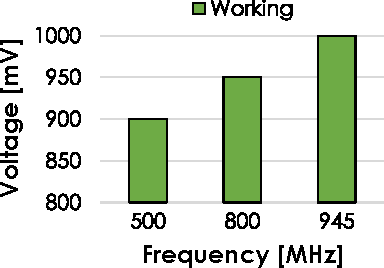
\includegraphics[width=0.35\textwidth]{Figures/GPU_characterization/DRAM_Guardband.pdf}
  \caption{Vega 10 - DRAM domain - Usable voltage for each frequency configuration.}
  \label{fig:DRAM_guardband}
\end{figure}

The result and the conclusion derived from the previous experiment was further verified with the execution of the kernel of Listing~\ref{lst:DRAMbitflip}. It is of extreme importance to validate if the use of lower voltage values induces data corruption on two edge cases: extreme use of part of the \acrshort{dram} and prolonged data storage. That said, the kernel was executed, and after time intervals of 1, 2, 5, 10, 30 minutes and 1, 2, 4 and 8 hours, the output data was retrieved and compared to the original set. Again, no perceptible change in the output was detected, further validating the previous result and assessing that the \acrshort{dram} can be successfully used with lower voltage levels. 

\subsection{Cache}
\label{sec:cache_guardband}

Figure~\ref{fig:CacheL2_guardband} presents the usable voltage interval at different frequency setups for both \acrshort{gpu}s. 
For the Vega 10 \acrshort{gpu}, no computation errors or crashes were observed at frequencies below $1530$~MHz. The \acrshort{gpu} operates correctly works at the lowest voltage across all the tested frequencies. 
Only for frequencies higher than $1530$MHz the  undervoltage resulted in the program crash. A critical observation is that no computation errors occur, meaning that this architectural component either works normally or makes the \acrshort{gpu} crash. This phenomenon is of significant importance to identify the root cause of failures: whenever it is observed a \acrshort{gpu} crash without prior computation errors, this may be the preeminent component causing it.
Furthermore, an increase of the \texttt{OPS} parameter allows for a higher amount of undervolt. Since this change only affects the stress over the DRAM-Cache controller (the number of cache accesses and hit-rate maintains the same), it can be concluded that it is the Cache-DRAM controller that limits the undervoltage range and not the memory elements of the cache. 

For the Radeon 5700 XT a similar behaviour is observed. For frequencies below $1600$~MHz, it is possible to use the \acrshort{gpu} at the lowest voltage without any computation errors or crashes being observed. For higher frequencies, when the voltage is reduced the most, the \acrshort{gpu} can crash. Increasing the value of the \texttt{OPS} parameter (decreasing Cache stress) increases the undervoltage capabilities. 


% \begin{figure}[htb]
%   \centering
%   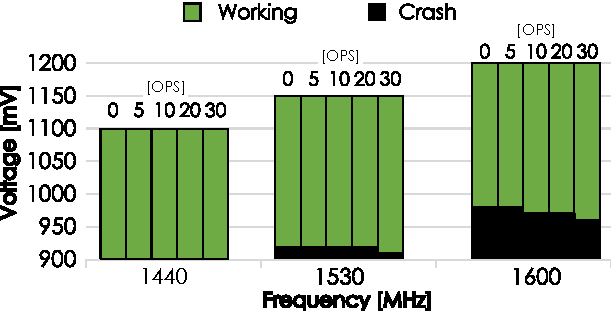
\includegraphics[width=0.5\textwidth]{Figures/GPU_characterization/CacheL2_guardband.pdf}
%   \caption{Core domain - Usable CacheL2 voltage for each frequency configuration with varying cache stress ($OPS$ value).}
%   \label{fig:CacheL2_guardband}
% \end{figure}

\begin{figure}[!htb]
    \centering
    \begin{subfigmatrix}{2}
      \label{fig:CacheL2_guardband}
      \subfigure[Vega 10.]{
        \centering
        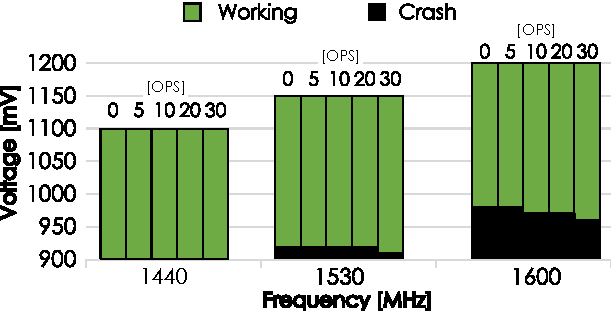
\includegraphics[width=0.49\textwidth]{Figures/GPU_characterization/CacheL2_guardband.pdf}
        \label{fig:Vega10-CacheL2_guardband}
      }
      \subfigure[Radeon 5700 XT.]{
        \centering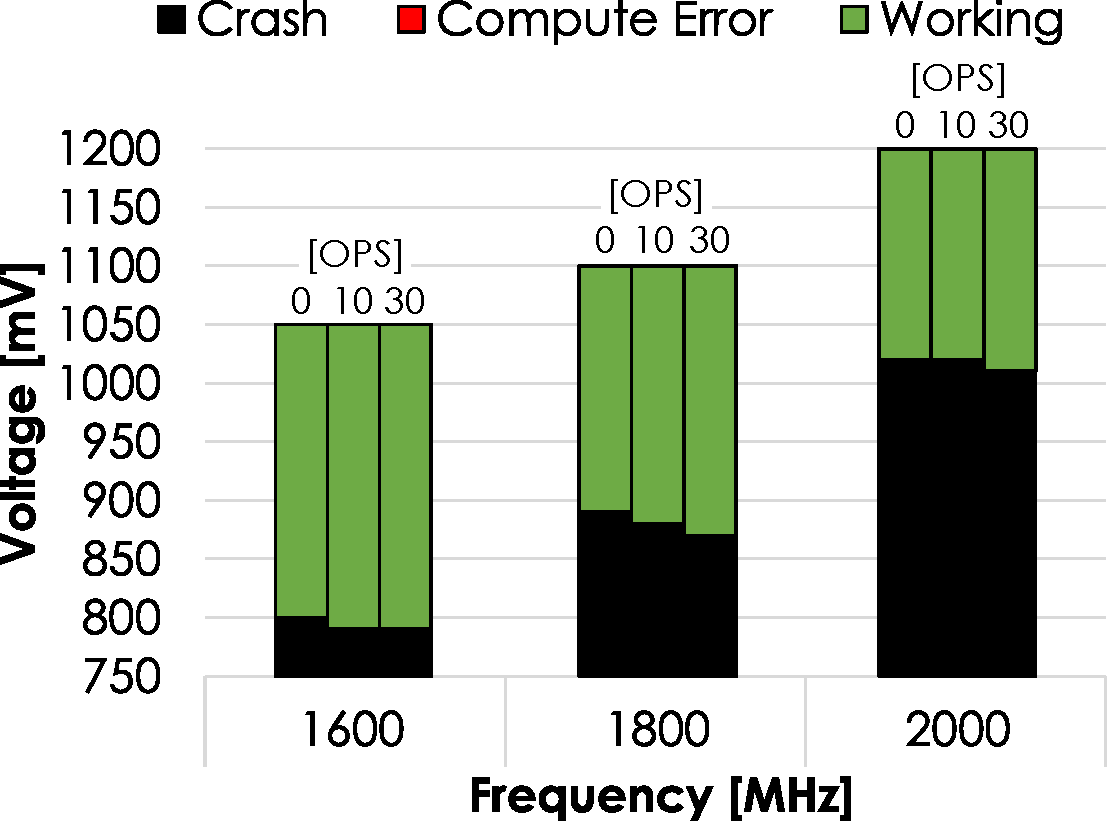
\includegraphics[width=0.42\textwidth]{Figures/GPU_characterization/5700XT-CacheL2_guardband_black.pdf}
        \label{fig:5700XT-CacheL2_guardband}
      }
    \end{subfigmatrix}
    \caption{Core domain - Cache L2 - Usable voltage for each frequency configuration with varying cache stress ($OPS$ value).}
\end{figure}


\subsection{Shared Memory}

\label{sec:cache_guardband}

The obtained voltage guardband results for the Shared Memory are presented in Figure~\ref{fig:SharedMemory_guardband}. Similarly with the Vega 10 Cache results, the benchmark's output was not affected by the applied undervoltage, for frequencies below $1530MHz$, with the \acrshort{gpu} operating correctly in the complete voltage range. For the frequencies above and equal to $1530MHz$, both computation errors and crashes occur. With the increase of the \texttt{OPS} parameter, from 0 to 10, it is observable that the \acrshort{gpu} starts allowing an increase of $10mV$ of undervoltage. This phenomenon indicates (and was also confirmed with \acrshort{gpu} counters) that with the reduction of the shared memory stress, the limiting factor to $V_{min}$ switches from the shared memory to the ALU (result confirmed ahead). The conclusion was further validated for the test at $1600MHz$, where increasing  \texttt{OPS} to 40 makes the \acrshort{gpu} start  crashing, meaning that the \acrshort{alu} is now the limiting factor.

For the Radeon 5700 XT, a similar behavior is found. However, even at the test with \texttt{OPS}=40 the limiting factor is still the Shared Memory. This is mainly due to a reduced memory interface and to a lower maximum memory bandwidth of the Radeon 5700 XT (256-bit and 448GB/s), contrasting to 2048-bit and 484GB/s of the Vega 10 \acrshort{gpu}.

% \begin{figure}[htb]
%   \centering
%   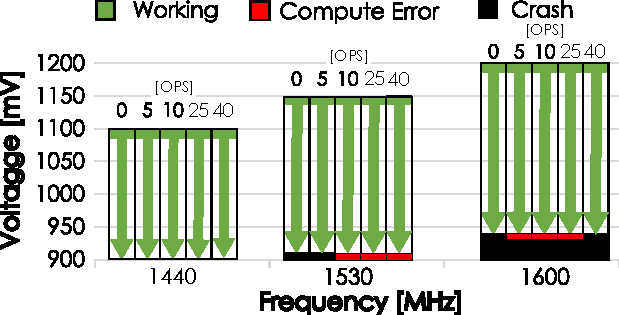
\includegraphics[width=0.5\textwidth]{Figures/GPU_characterization/SharedMemory_guardband.pdf}
%   \caption{Vega 10 - Core domain - Shared Memory - Usable voltage for each frequency configuration with varying shared memory stress ($OPS$ value).}
%   \label{fig:SharedMemory_guardband}
% \end{figure}

\begin{figure}[!htb]
    \centering
    \begin{subfigmatrix}{2}
      \label{fig:SharedMemory_guardband}
      \subfigure[Vega 10.]{
        \centering
        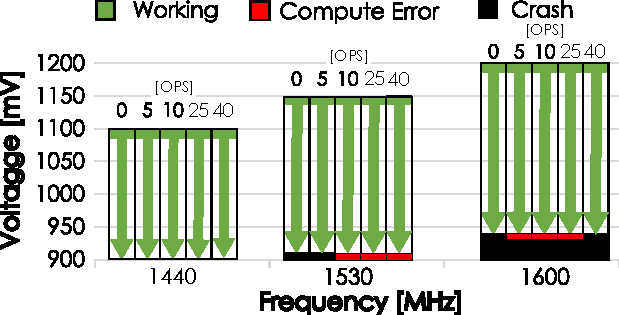
\includegraphics[width=0.49\textwidth]{Figures/GPU_characterization/SharedMemory_guardband.pdf}
        \label{fig:Vega10-SharedMemory_guardband}
      }
      \subfigure[Radeon 5700 XT.]{
        \centering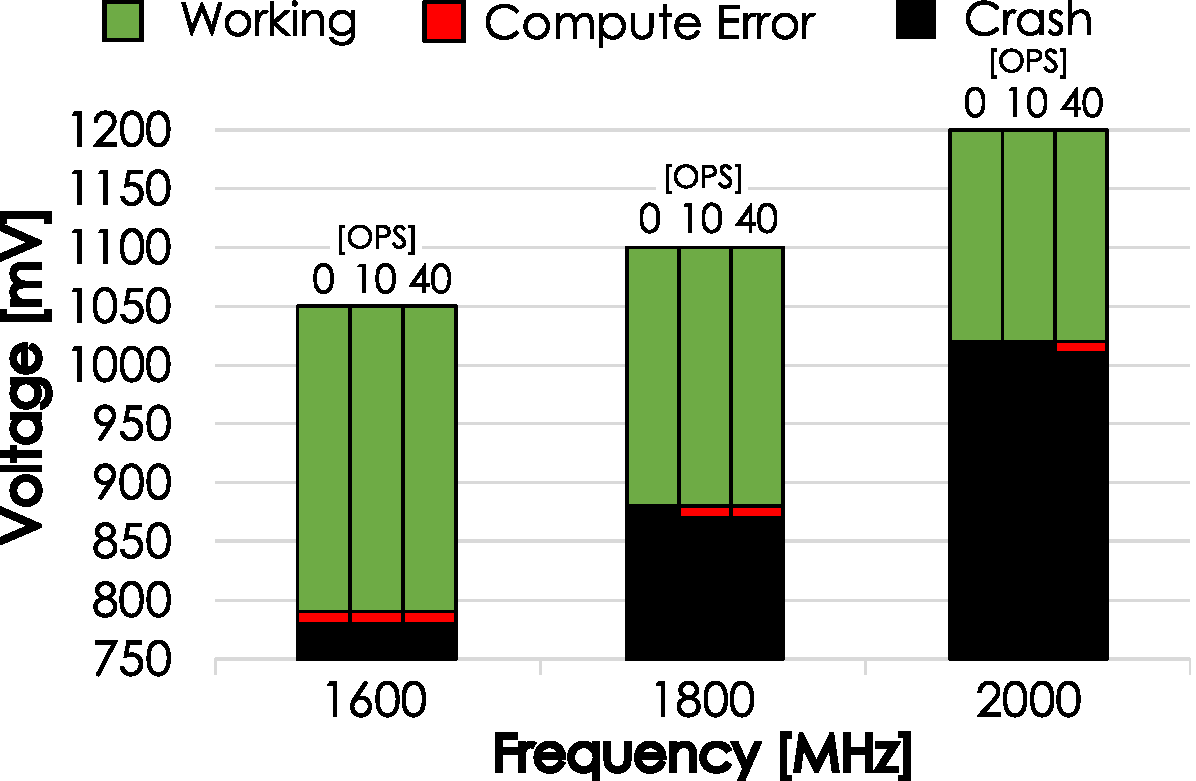
\includegraphics[width=0.42\textwidth]{Figures/GPU_characterization/5700XT-SharedMemory_Guardband.pdf}
        \label{fig:5700XT-SharedMemory_guardband}
      }
    \end{subfigmatrix}
    \caption{Core domain - Shared Memory - Usable voltage range for each frequency configuration with varying shared memory stress ($OPS$ parameter).}
\end{figure}

\subsection{Arithmetic and Logic Unit}

\label{sec:cmac_guardband}

Figure~\ref{fig:MAC_guardband} represents the usable undervoltage range for the \acrshort{alu} benchmark. This benchmark was executed either for integer and for the several different floating-point precisions available on each \acrshort{gpu}. 

On the Vega 10 \acrshort{gpu}, and in all considered scenarios using an operating frequency below $1440$~MHz, the benchmark was successfully run for all voltage values. For higher frequencies, it is observed that some computation errors start appearing after a certain amount of undervoltage. In particular, the \acrshort{gpu} crashes if a further undervoltage level is applied. 
It is also observable that the voltage margin increases with the operating frequency, from around $170$mV for $1440$~MHz to around $210$mV for $1600$~MHz (values for single-precision floating-point). On the Radeon 5700 XT \acrshort{gpu}, the \acrshort{alu} benchmark works  correctly independently of the applied voltage, for frequencies below $1600$~MHz. At higher frequencies, and  similarly to what happens with the Vega 10, a computation error margin exists when undervolting, before the occurrence of crashes. Overall, the Radeon 5700 XT \acrshort{gpu} allows more than $200$mV of safe undervoltage across the complete frequency spectrum.

In general, it was observed that the operands that are "easier" to compute (namely the integer and half-precision) allow the highest amount of undervoltage, not being the computation of those the limiting factor of the \acrshort{alu}. 
In fact, it was expected that whe  comparing floating-point single precision with double precision, the second would have a worse undervolting capabilities, due to having the double amount of bits to compute. However, the opposite relation was observed, with double-precision allowing for an extra $10$ to $20mV$ of undervoltage (when comparing the crash point). This leads us to conclude that single and double floating-point computation is not performed in the same way. In fact, although most  \acrshort{risc} microprocessors are pipelined, the way the pipeline stages are divided is not non the same. It is reasonable to expect that the double-precision computation is split among more clock cycles than the single precision, allowing for an extra relaxation of the timing constraints on that data path.

The dependencies effect also varied from integer to floating-point operation. In the first case, the code's dependencies do not affect the size of the voltage margin. In the second case, the existence of dependencies in the code reduces the voltage margin's size. In general, when compared with the setup with no dependencies (\texttt{d=0}), the undervoltage range of the benchmark configuration that represent the general case (\texttt{d=3} - see Listings~\ref{lst:MACbench}) is reduced by $10$mV. 

% \begin{figure}[htb]
%   \centering
%   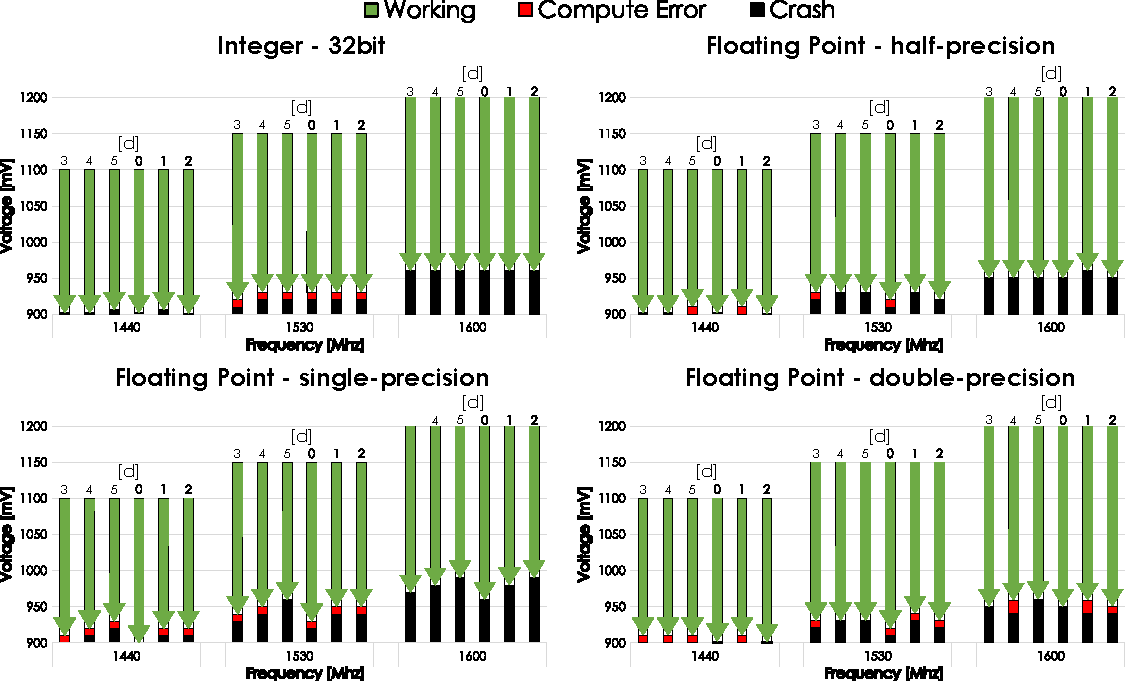
\includegraphics[width=1\textwidth]{Figures/GPU_characterization/MAC_Guardband.pdf}
%   \caption{Core domain - Usable ALU-MAC voltage for the different data types and operand's precision.}
%   \label{fig:MAC_guardband}
% \end{figure}

\begin{figure}[!htb]
    \centering
    \begin{subfigmatrix}{2}
      \label{fig:MAC_guardband}
      \subfigure[Vega 10.]{
        \centering
        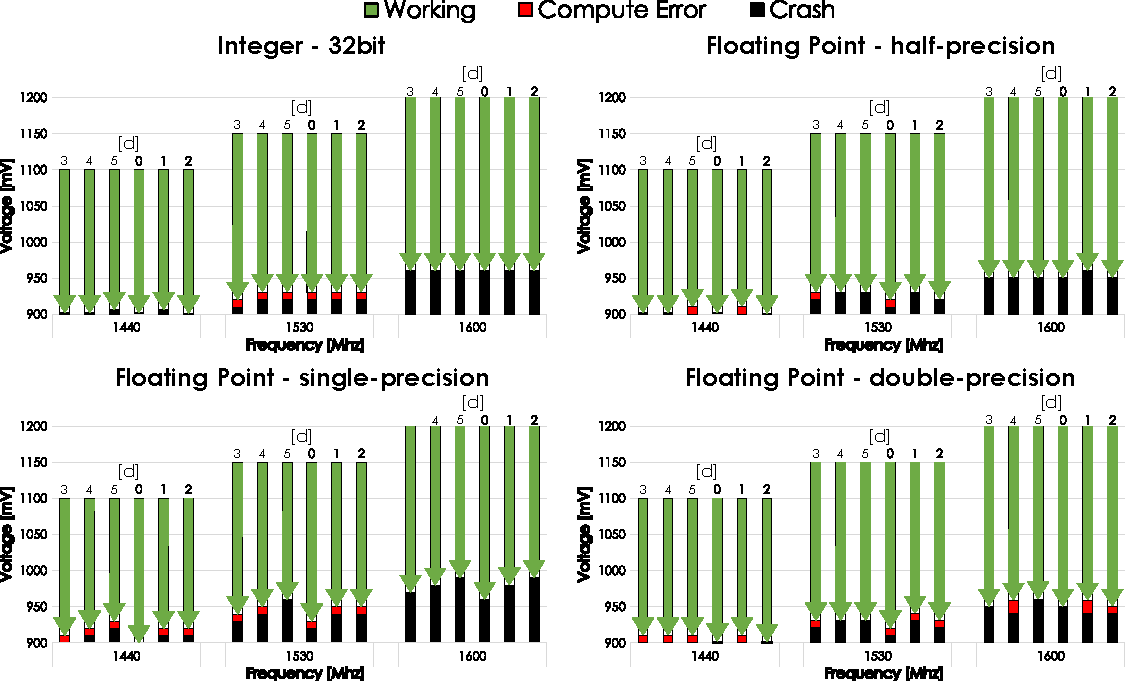
\includegraphics[width=0.97\textwidth]{Figures/GPU_characterization/MAC_Guardband.pdf}
        \label{fig:Vega10-MAC_guardband}
      }
      \subfigure[Radeon 5700 XT.]{
        \centering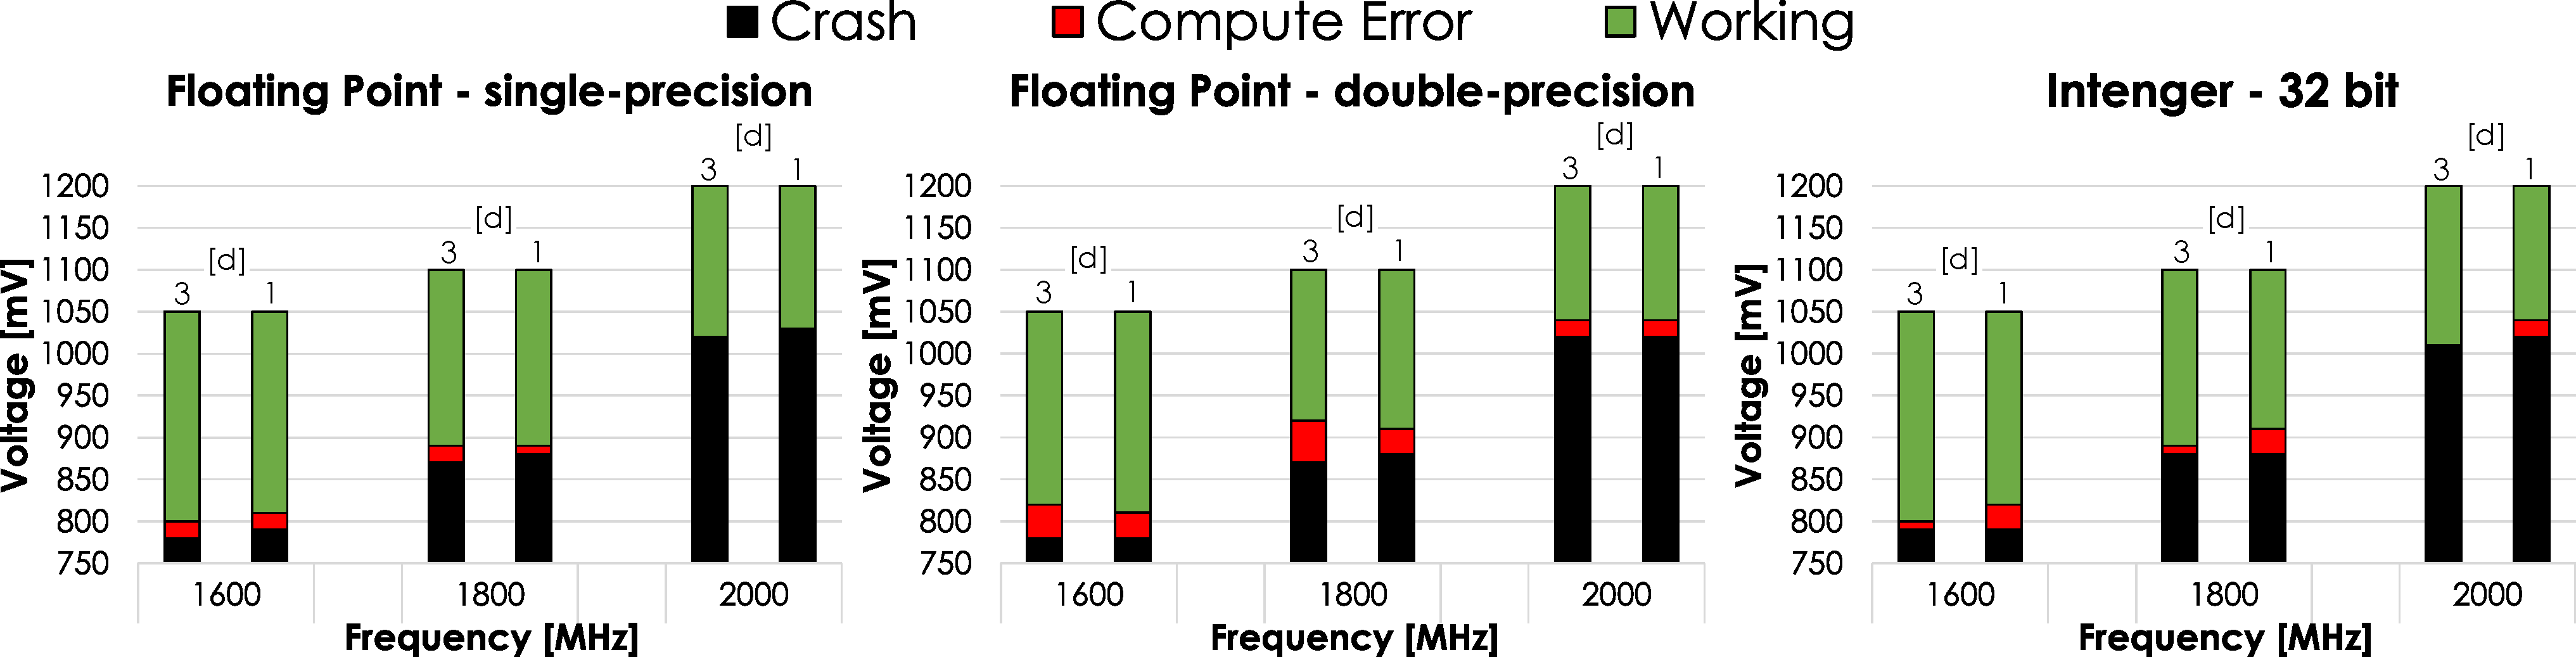
\includegraphics[width=0.97\textwidth]{Figures/GPU_characterization/5700XT-MAC_Guardband.pdf}
        \label{fig:5700XT-MAC_guardband}
      }
    \end{subfigmatrix}
    \caption{Core domain - ALU-MAC - Usable voltage margins for the different data types and operand's precision.}
\end{figure}



\subsection{Non-linear Operations}

The special function unit (\acrshort{sfu}) was also tested for floating-point operation of single and double-precision, with the results being presented in Figure~\ref{fig:SFU_guardband}. Similarly with the results of the \acrshort{mac} operation, double precision allows a further $10$ to $20mV$ of valid undervoltage, when  compared to single precision. Overall, this unit's voltage guardband is similar to the one of the \acrshort{alu} on the \acrshort{mac} operation. 



\begin{figure}[!htb]
    \centering
    \begin{subfigmatrix}{2}
      \label{fig:SFU_guardband}
      \subfigure[Vega 10.]{
        \centering
        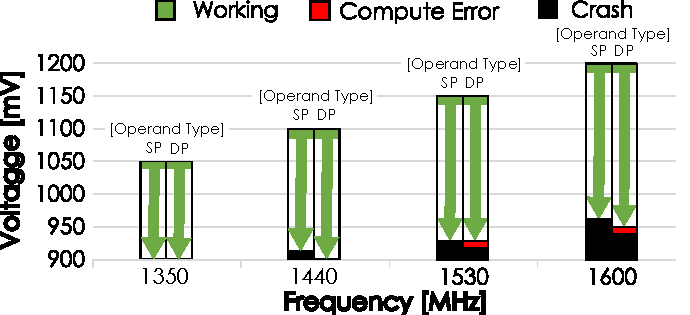
\includegraphics[width=0.44\textwidth]{Figures/GPU_characterization/SFU_guardband.pdf}
        \label{fig:Vega10-SFU_guardband}
      }
      \subfigure[Radeon 5700 XT.]{
        \centering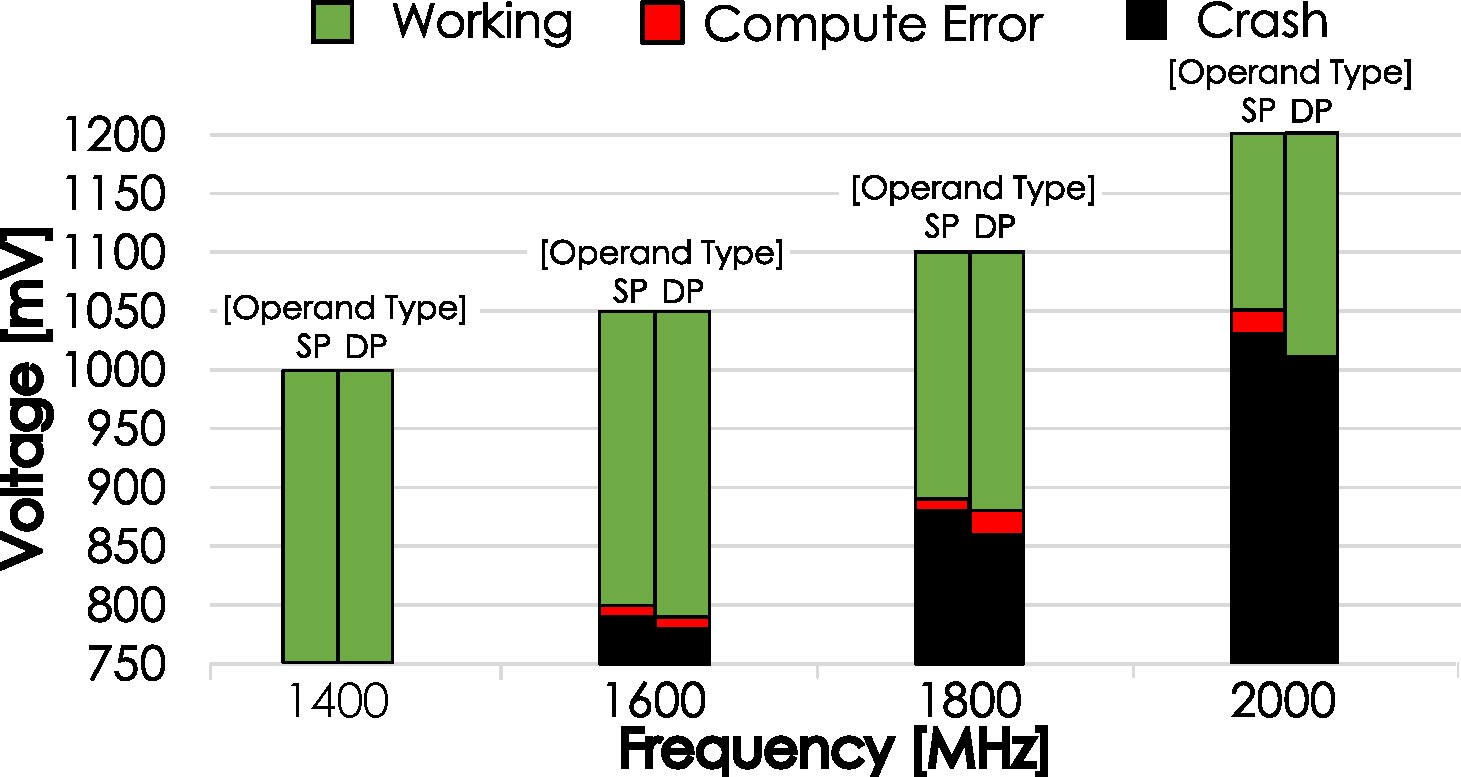
\includegraphics[width=0.46\textwidth]{Figures/GPU_characterization/5700XT-SFU_Guardband.pdf}
        \label{fig:5700XT-SFU_guardband}
      }
    \end{subfigmatrix}
    \caption{Core domain - Special Function Unit - Usable voltage for each frequency configuration with varying operand type: SP - Single Precision Floating-Point, DP - Double Precision Floating-Point.}
\end{figure}

\subsection{Branches}

Figure~\ref{fig:Branches_guardband} presents the results of the branches test. As it can be observed, the number of branches on the kernel did not affect the voltage guardband's size, with all configurations (for each operating frequency) allowing the same degree of undervoltage.
Hence, the obtained result allowed the conclusion that branch miss-prediction does not negatively impact $V_{min}$. It is expected that, independently of the number of branches that a kernel has, the limiting factor to $V_{min}$ is the type of operations being executed, leading to computational errors and eventually to \acrshort{gpu} crash as determined by the other experiments.

% \begin{figure}[htb]
%   \centering
%   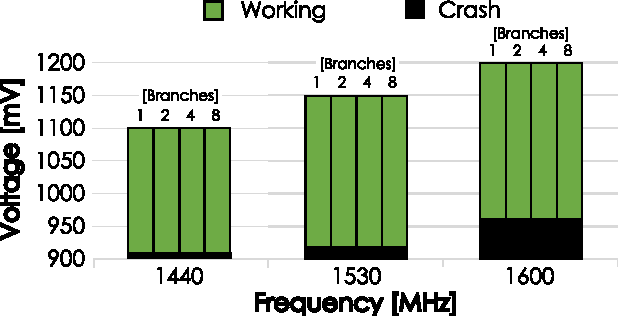
\includegraphics[width=0.67\textwidth]{Figures/GPU_characterization/Branches_guardband_3.pdf}
%   \caption{Vega 10 - Core domain - Usable Branches voltage for each frequency configuration with varying number of branches per iteration.}
%   \label{fig:Branches_guardband}
% \end{figure}

\begin{figure}[!htb]
    \centering
    \begin{subfigmatrix}{2}
      \label{fig:Branches_guardband}
      \subfigure[Vega 10.]{
        \centering
        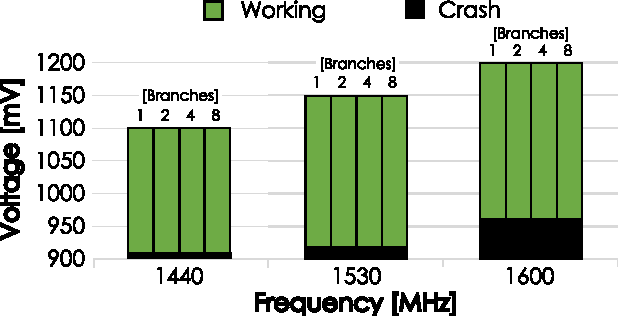
\includegraphics[width=0.46\textwidth]{Figures/GPU_characterization/Branches_guardband_3.pdf}
        \label{fig:Vega10-Branches_guardband}
      }
      \subfigure[Radeon 5700 XT.]{
        \centering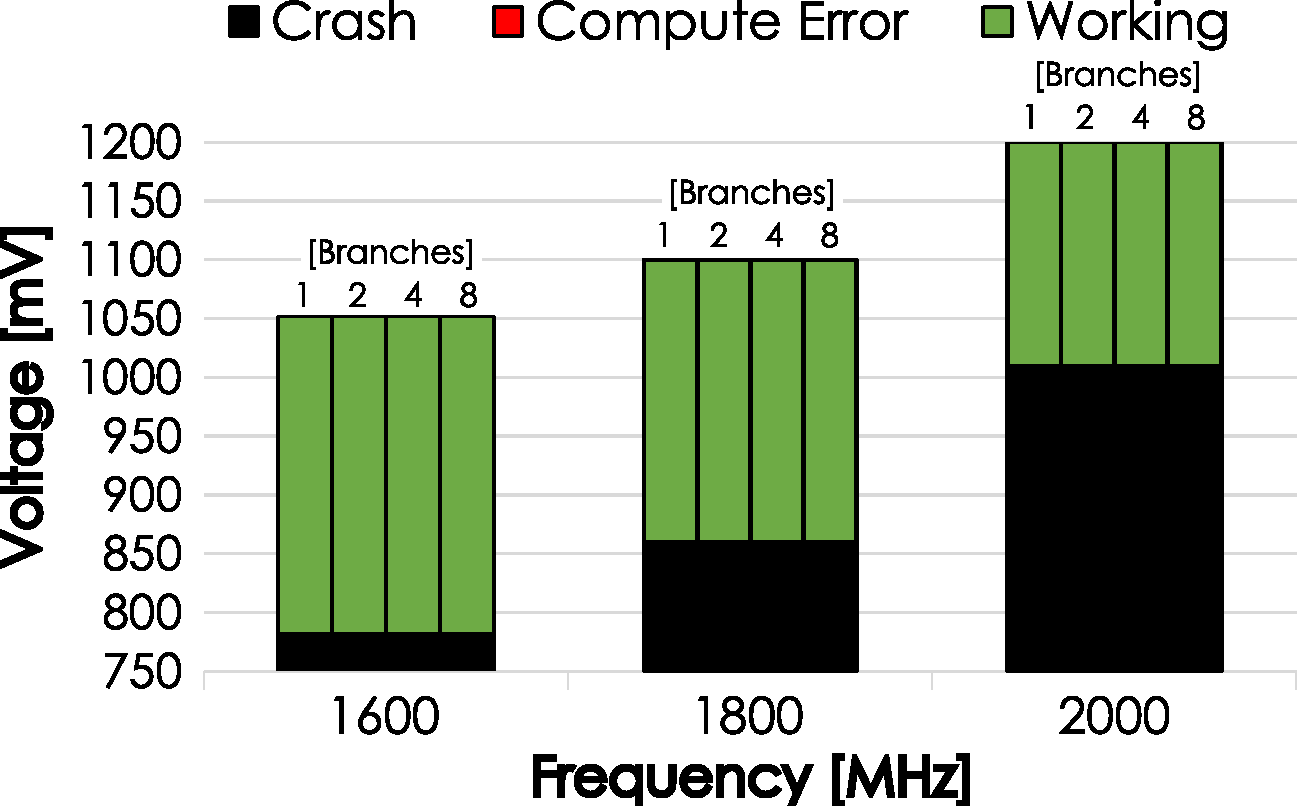
\includegraphics[width=0.44\textwidth]{Figures/GPU_characterization/5700XT-Branches_guardband.pdf}
        \label{fig:5700XT-Branches_guardband}
      }
    \end{subfigmatrix}
    \caption{Core domain - Branches - Usable voltage for each frequency configuration with varying number of branches per iteration.}
\end{figure}

\subsection{Reduction}

Figure~\ref{fig:Reduction_guardband} presents the usable voltage range for the \texttt{reduction} benchmark. As can be seen, due to the high pressure exercised on the cache by this benchmark, the minimum usable voltage coincides with the one already measured for the Cache benchmark. The \acrshort{alu} benchmark can explain the several data types range of compute errors and $V_{min}$ value differences, with double-precision floating-point having a bigger margin of computational errors (on the Radeon 5700 XT) and overall reduced voltage guardband at the higher frequencies on both \acrshort{gpu}s.

% \begin{figure}[htb]
%   \centering
%   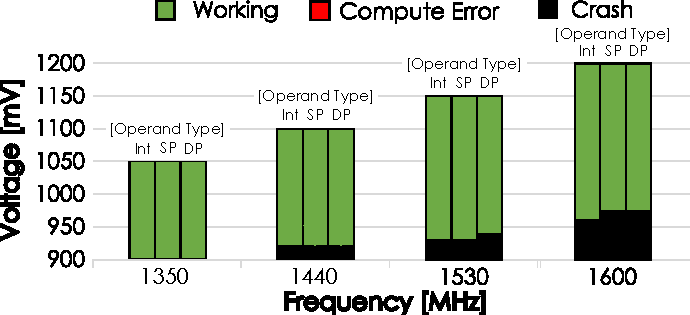
\includegraphics[width=0.59\textwidth]{Figures/GPU_characterization/Reduction_guardband.pdf}
%   \caption{Vega 10 - Core domain - Reduction benchmark - Usable voltage for each frequency configuration with varying operand type: Int - 32-bit Integer, SP - Single Precision Floating-Point, DP - Double Precision Floating-Point.}
%   \label{fig:Reduction_guardband}
% \end{figure}

\begin{figure}[!htb]
    \centering
    \begin{subfigmatrix}{2}
      \label{fig:Reduction_guardband}
      \subfigure[Vega 10.]{
        \centering
        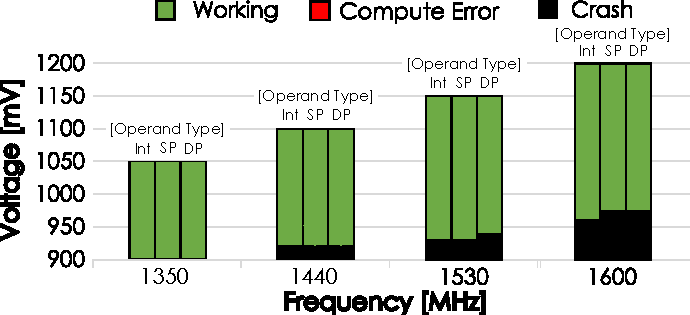
\includegraphics[width=0.42\textwidth]{Figures/GPU_characterization/Reduction_guardband.pdf}
        \label{fig:Vega10-Reduction_guardband}
      }
      \subfigure[Radeon 5700 XT.]{
        \centering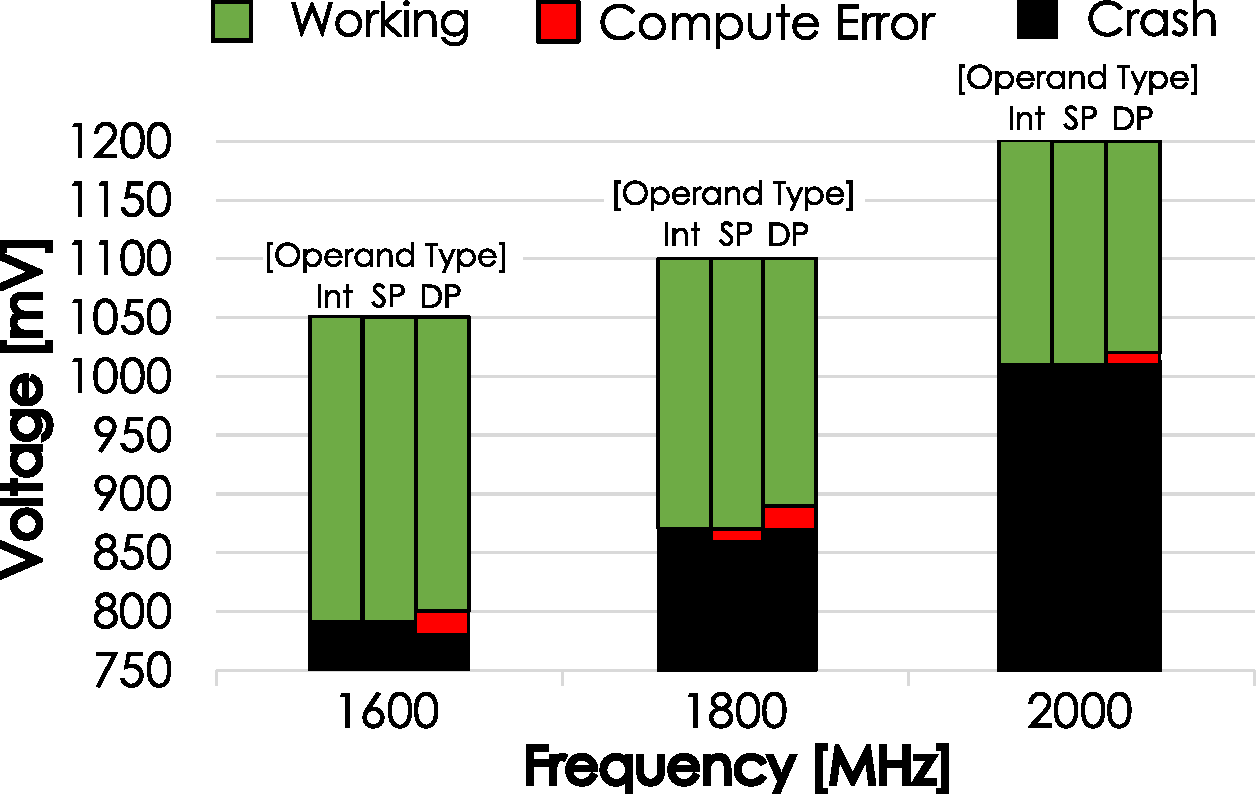
\includegraphics[width=0.47\textwidth]{Figures/GPU_characterization/5700XT-Reduction_Guardband.pdf}
        \label{fig:5700XT-Reduction_guardband}
      }
    \end{subfigmatrix}
    \caption{Core domain - Reduction benchmark - Usable voltage for each frequency configuration with varying operand type: Int - 32-bit Integer, SP - Single Precision Floating-Point, DP - Double Precision Floating-Point.}
\end{figure}


\subsection{General Comments and Remarks}


Figure~3.9 presents a comprehensive comparison of the valid voltage ranges for all the considered architectural components of both \acrshort{gpu}s. 
The general observation is that the CacheL2 and the \acrshort{alu} are the two components that tend to compromise the undervoltage capabilities. CacheL2 affects the kernels that are more memory intensive, while the \acrshort{alu} limits those that are more compute-intensive, either with linear or special non-linear operations. 

In more detail, the results of both benchmarks that test the \acrshort{alu} are similar. This allows concluding one of two things, either  there are two similar critical paths (in terms of timing constraints) on both the linear and non-linear data paths, or the critical path is at the beginning of the  \acrshort{alu} where the operands are forward to the appropriate computational unit. Although it is not possible to assess which preposition is the correct one, the second explanation tends to be more credible.

In general, even though two completely different \acrshort{gpu} architectures are under test, the general behavior of both is similar. At the lower frequencies available, the minimum voltage can be safely applied without the existence of computation errors or crashes. The utilization of undervoltage for higher frequencies will depend on which components the application being executed stresses the most. Across all frequencies, both \acrshort{gpu}s allow for more than $20\%$ of safe undervoltage, being a considerable amount to be explored in the following section.


% \begin{figure}[h]
%     \centering
%         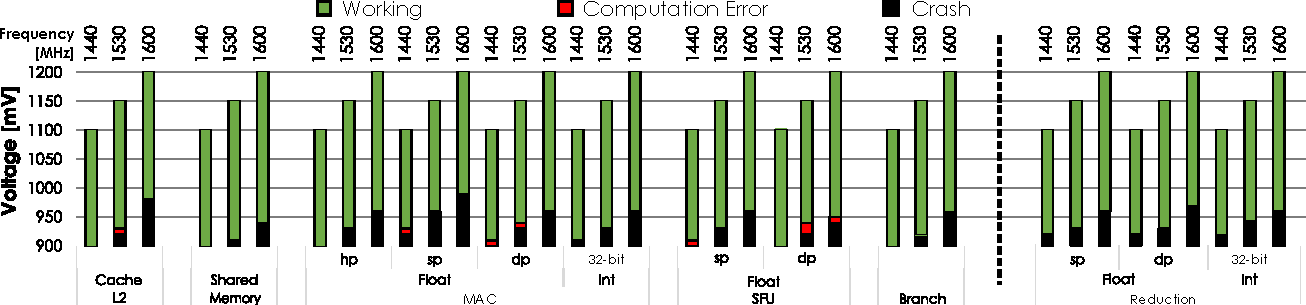
\includegraphics[width=1\textwidth]{Figures/GPU_characterization/Comparison_Guardband.pdf}
%         \caption{Comparison of usable GPU core voltage ranges for all the considered architectural components of the GPU.}
%     \label{fig:Guardband_comparison}
% \end{figure}

% \begin{figure}[!htb]
%     \centering
%     \begin{subfigmatrix}{2}
%       \label{fig:Guardband_comparison}
%       \subfigure[Vega 10.]{
%         \centering
%         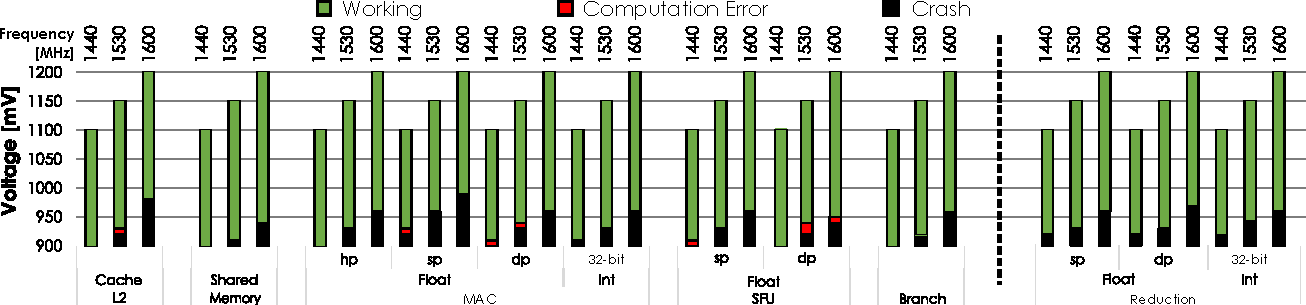
\includegraphics[width=0.95\textwidth]{Figures/GPU_characterization/Comparison_Guardband.pdf}
%         \label{fig:Vega10-Comparison_Guardband}
%       }
%       \subfigure[Radeon 5700 XT.]{
%         \centering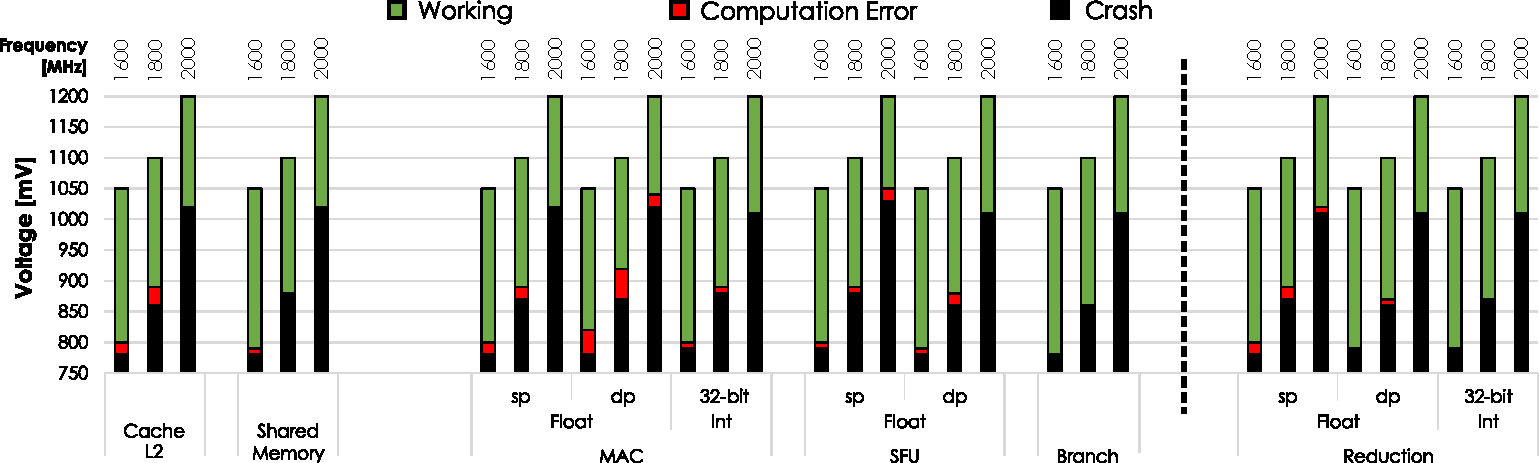
\includegraphics[width=0.95\textwidth]{Figures/GPU_characterization/5700XT-Comparison_Guardband.pdf}
%         \label{fig:5700XT-Comparison_Guardband}
%       }
%     \end{subfigmatrix}
%     \caption{Comparison of usable GPU core voltage ranges for all the considered architectural components of the GPU.}
% \end{figure}

\begin{sidewaysfigure}[!htb]
    \centering
    \begin{subfigmatrix}{2}
      \label{fig:Comparison_Guardband}
      \subfigure[Vega 10.]{
        \centering
        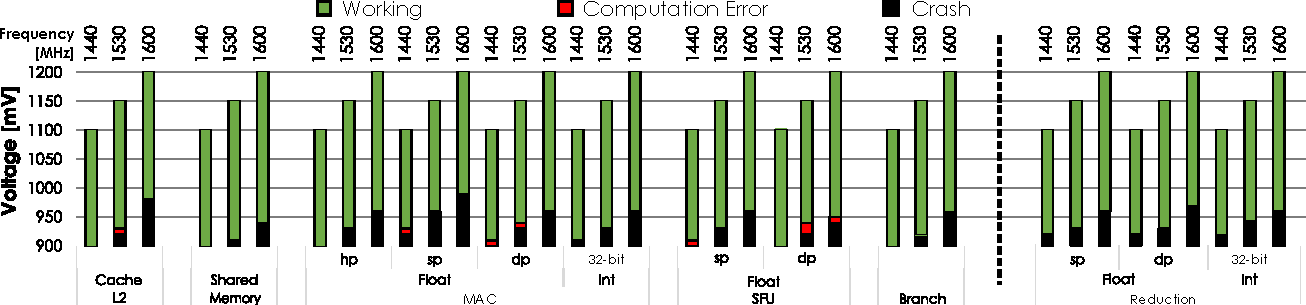
\includegraphics[width=0.95\textwidth]{Figures/GPU_characterization/Comparison_Guardband.pdf}
        \label{fig:Vega10-Comparison_Guardband}
      }
      \subfigure[Radeon 5700 XT.]{
        \centering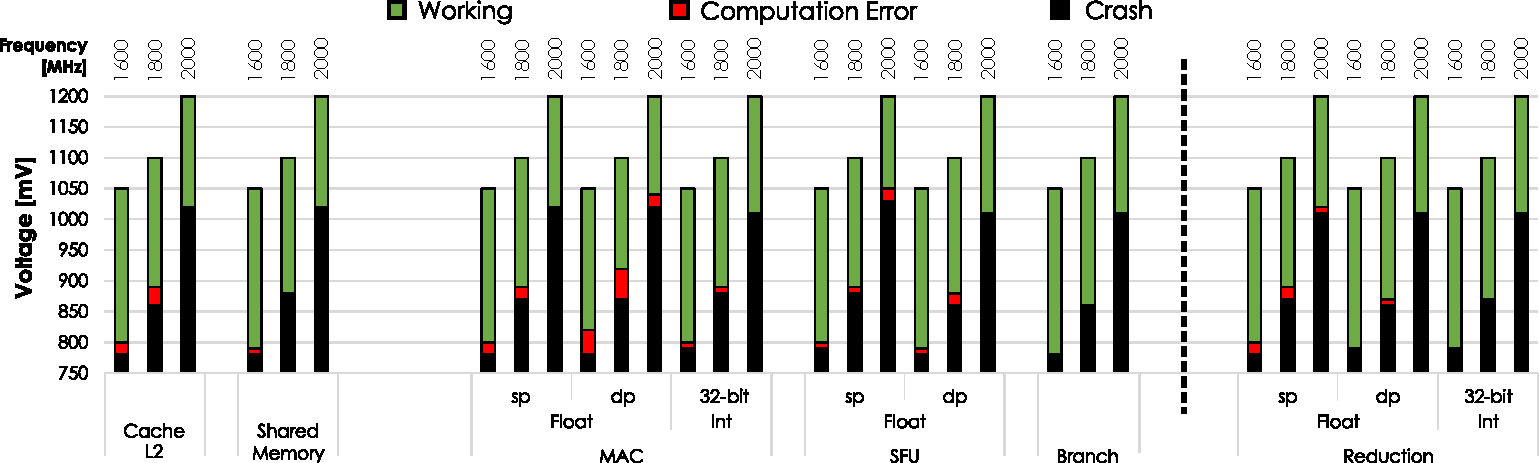
\includegraphics[width=0.95\textwidth]{Figures/GPU_characterization/5700XT-Comparison_Guardband.pdf}
        \label{fig:5700XT-Comparison_Guardband}
      }
    \end{subfigmatrix}
    \caption{Comparison of usable GPU core voltage ranges for all the considered architectural components of the GPU.}
\end{sidewaysfigure}


\clearpage

%%%%%%%%%%%%%%%%%%%%%%%%%%%%%%%%%%%%%%%%%%%%%%%%%%%%%%%%%%%%%%%%%%%%%%%%
\section{Effect of a decoupled V-F scaling on performance and energy consumption}
\label{sec:gpu_behaviour}


As it was observed in the previous section, the \acrshort{gpu} behavior to V-F scaling depends on the stressed components. Having explored and established the usable V-F  pairs, this section presents the energy-performance charts and the \acrshort{edp} heat-maps for each of the tested benchmarks. In particular, this section's results indicate the maximum attainable improvement on each component and acts as a target optimization for subsequent analysis using complete applications. 



For an easier understanding of the obtained results, the following charts only represent the data-points that correspond to voltages equal-to and lower-than the default voltage of each frequency level (no interesting data is found at higher voltage levels), with each data point representing a $50mV$ undervoltage in relation to the previous one.
Furthermore, the presented performance, energy consumption, and energy-delay product charts are normalized to the results achieved with the highest core frequency and default voltage ( Vega 10 - \{$1600$~MHz; $1.2$V\} and Radeon 5700 XT - \{$2000$~MHz; $1.2$V\}). As such, a smaller number indicates an improvement in relation to that configuration. 

\subsection{DRAM}

Figure~\ref{fig:DRAM_behaviour} illustrates the normalized performance and energy consumption of the conceived \acrshort{dram} benchmark (see Listings~\ref{lst:DRAMbench}) when varying the \texttt{OPS} parameter between 0 and 50 operations for the \acrshort{dram} \acrshort{dvfs} domain, normalized to the highest \acrshort{dram} \acrshort{dvfs} V-F configuration - \{950MHz, 1V\}.

This experiment shows that, for all \texttt{OPS} values ($0$ to $50$), the highest DRAM frequency delivers not only the best performance but also the lowest energy consumption. Moreover, undervolting the DRAM at that frequency did not result in a relevant reduction in the total GPU energy consumption, leading to the conclusion that the weight of \acrshort{dram} in the GPU energy consumption is not significant in relation to the \textit{Core} energy consumption. In accordance, the highest \acrshort{dram} frequency will be hence-forwardly considered, guaranteeing the maximum performance and leaving the voltage control for the automatic DVFS system.


\begin{figure}[htb]
  \centering
  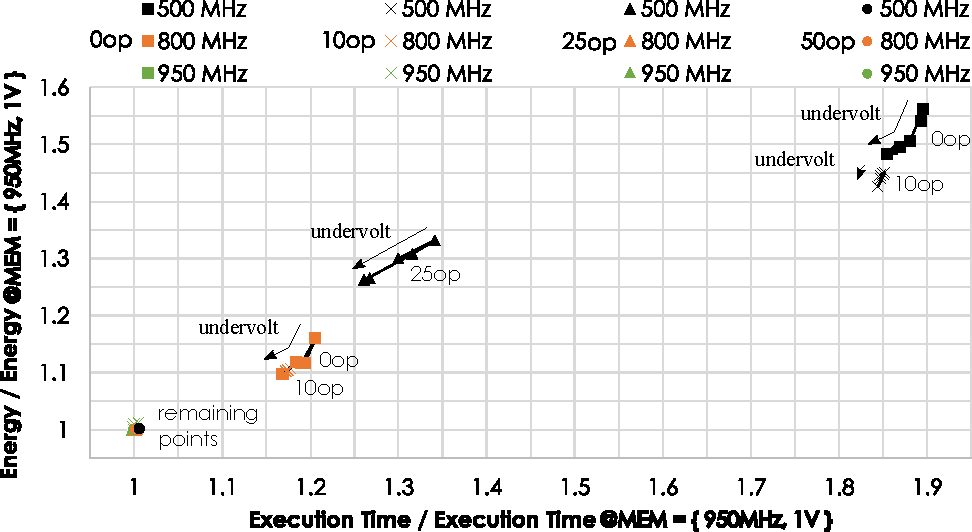
\includegraphics[width=0.75\textwidth]{Figures/GPU_characterization/DRAM_behaviour.pdf}
  \caption{Vega 10 - DRAM domain - DRAM benchmark - Normalized energy consumption and execution time. Each connected data point represents a $50mV$ undervoltage in relation to the previous one.}
  \label{fig:DRAM_behaviour}
\end{figure}

A collateral experiment was also conducted to evaluate any possible cross-relation between the applied V-F setup at the Core domain when executing the \acrshort{dram} benchmark with a variable amount of stress in memory bounded kernels. Figure~\ref{fig:DRAM_Corebehaviour} illustrates the normalized performance and energy consumption, with varying \texttt{OPS} parameter between 0 and 50 operations (see Listings~\ref{lst:DRAMbench}). For this benchmark, it is not relevant to determine the minimum usable voltage, since that value will be defined by the type of operations being performed on the Core. The objective is to determine the configuration that offers the best energy efficiency for kernels that are memory bounded.  

The experiment shows that for memory bounded kernels (\texttt{OPS} values $0$ and $10$), performing frequency scaling at the core domain does not change the computation time. However, it significantly impacts the energy consumption (going from the highest frequency to the lowest yields a $54.2\%$ reduction on energy consumption). For the case of a kernel that is not memory bounded  (\texttt{OPS} $=25$), the benefit of exploring non-conventional V-F pairs becomes clear. However, as stated, the optimization of the V-F pairs for compute bounded kernels depends on the type of operations being performed in the \acrshort{alu}, analyzed in the following sections.

\begin{figure}[htb]
  \centering
  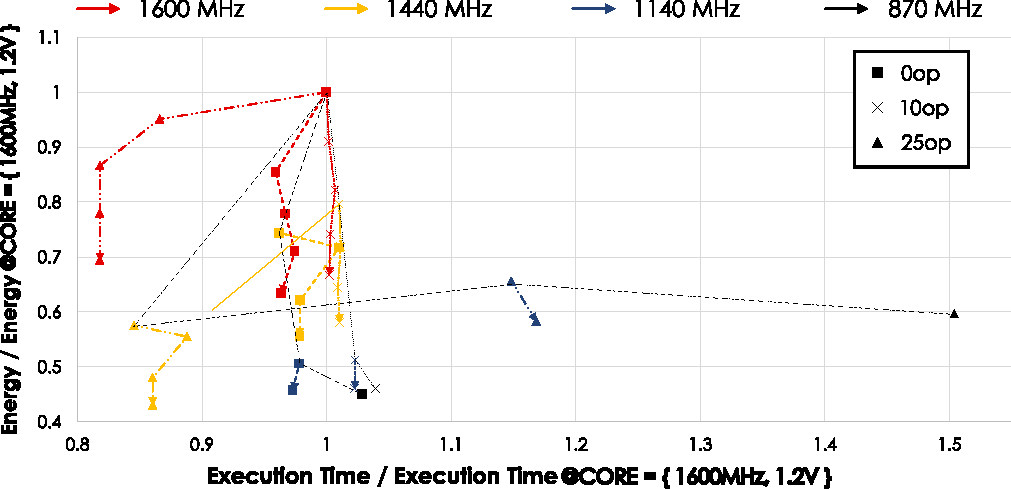
\includegraphics[width=0.75\textwidth]{Figures/GPU_characterization/DRAM_Core_domain_behaviour.pdf}
  \caption{Vega 10 - Core domain - DRAM - Normalized energy consumption and execution time. The dashed line connects the default V-F configurations and each connected data point represents a $50mV$ undervoltage in relation to the previous one.}
  \label{fig:DRAM_Corebehaviour}
\end{figure}


\subsection{Cache and Shared Memory}

\label{sec:cache_sm__behaviour}

Figure~\ref{fig:cache_behaviour} and \ref{fig:sm_behaviour} presents the normalized energy consumption and execution time for different V-F setups for the cache and shared memory benchmarks, respectively. Acting on core domain, the normalization of the present and all subsequent benchmark is done to the highest V-F configuration available:Vega 10 - \{$1600$~MHz; $1.2$V\} and Radeon 5700 XT - \{$2000$~MHz; $1.2$V\}.

In what concerns the energy and performance variations, it was observed that performing voltage the conventional scaling (using the default frequency - dashed line) provides an energy consumption as high as $46\% $ for Vega 10 \acrshort{gpu} and $30\% $ for Radeon 5700 XT \acrshort{gpu}. However, this also introduces a performance degradation of $61\%$ on both \acrshort{gpu}s. 

As it was refered before, the advantage of performing non-conventional DVFS becomes apparent by allowing for energy reduction without any performance degradation. For example, the Vega 10 running at \{1600MHz ; 1V\} allows an energy reduction of $36\%$ while still being a peak performance.
In the Radeon 5700 XT case, the use of non-conventional V-F pairs yields a minimum energy consumption that is even lower than the most energy-saving default V-F configuration, with the configuration of \{1800MHz ; 0.8V\} achieving an energy consumption reduction of $41\%$ with only a $10\%$ performance downgrade. This energy consumption reduction is twice as big as the one achieved at the most energy-saving default V-F configuration.
% In this case, it is possible to run the GPU Core at $1600$ MHz and $1000$ mV, thus achieving an energy reduction of $35.7\%$ with no performance degradation. The commented results are related to the cache benchmark. 
The results of the shared memory are similar.

\begin{figure}[!htb]
    \centering
    \begin{subfigmatrix}{2}
      \label{fig:cache_behaviour}
      \subfigure[Vega 10.]{
        \centering
        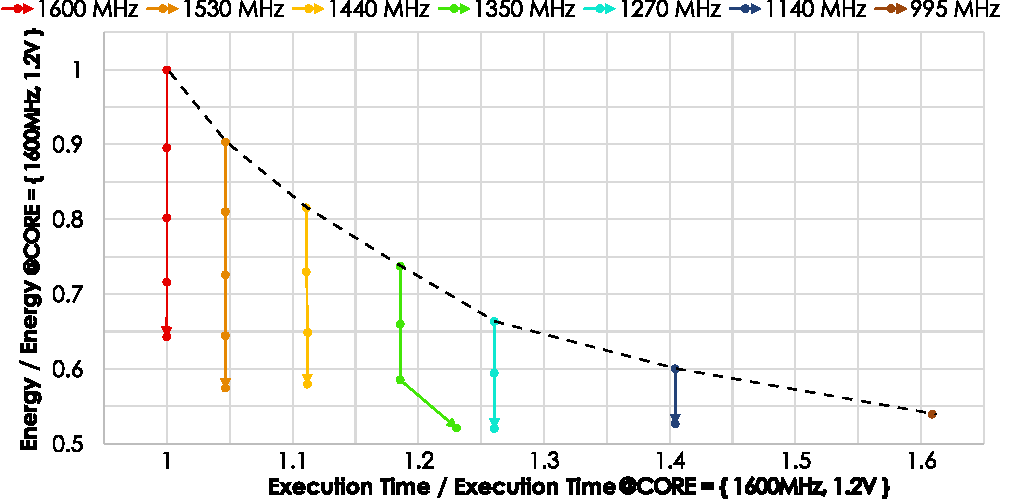
\includegraphics[width=0.45\textwidth]{Figures/GPU_characterization/CacheL2_behaviour_0op_no_marks.pdf}
        \label{fig:Vega10-cache_behaviour}
      }
      \subfigure[Radeon 5700 XT.]{
        \centering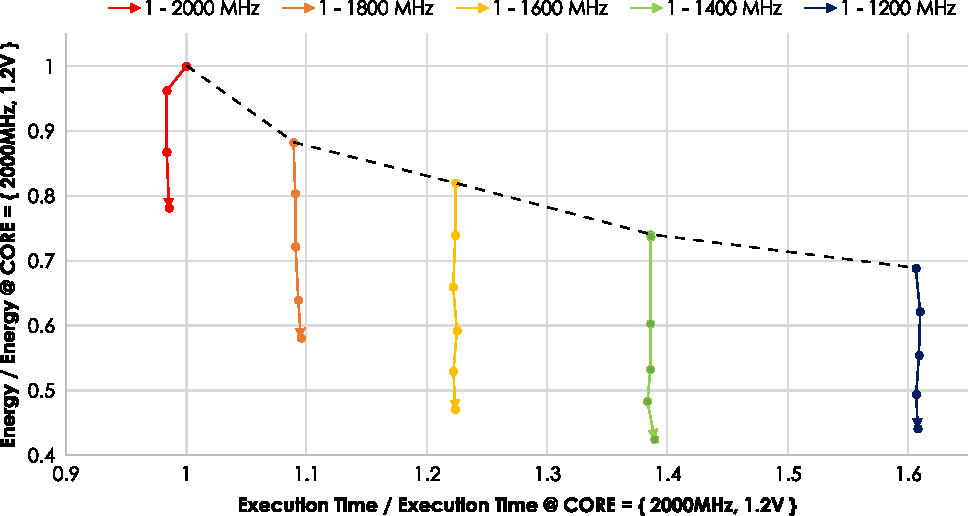
\includegraphics[width=0.45\textwidth]{Figures/GPU_characterization/5700XT-CacheL2_behaviour_0op.pdf}
        \label{fig:5700XT-cache_behaviour}
      }
    \end{subfigmatrix}
    \caption{Core domain - Cache L2 - Normalized energy and performance variations with \texttt{OPS}=0. The dashed line connects the default F-V configurations.}
\end{figure}

% \begin{figure}[htb]
%   \centering
%   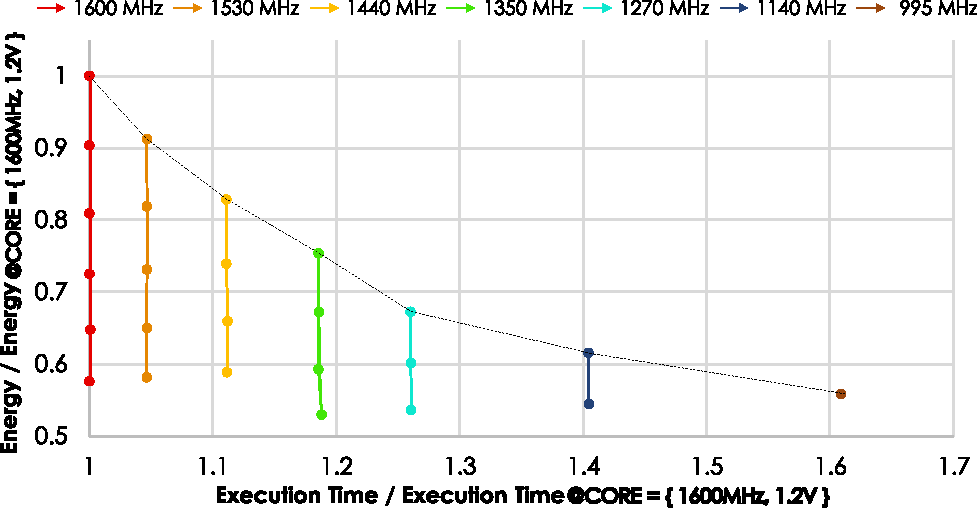
\includegraphics[width=0.5\textwidth]{Figures/GPU_characterization/SharedMemory_behaviour.pdf}
%   \caption{Vega 10 - Core domain - Shared Memory - Normalized energy consumption and execution time. The dashed line connects the default F-V configurations and each connected data point represents a $50mV$ undervoltage in relation to the previous one.}
%   \label{fig:sm_behaviour}
% \end{figure}



% \begin{figure}[!htb]
%   \begin{subfigmatrix}{2}
%     \subfigure[Cache]{\label{fig:cacheL2_behaviour}\includegraphics[width=0.48\textwidth]{}}
%     \subfigure[Shared Memory]{\label{fig:sm_behaviour}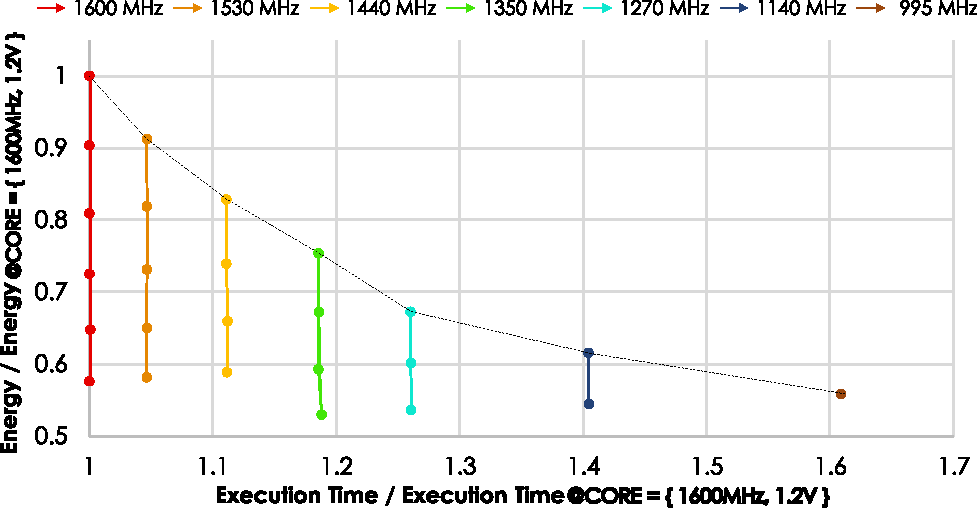
\includegraphics[width=0.46\textwidth]{Figures/GPU_characterization/SharedMemory_behaviour.pdf}}
%   \end{subfigmatrix}
%   \caption{Core domain - Normalized energy and performance variations for \texttt{OPS}=0. The  values shown in the left figure represent the applied core voltage and the dashed line connects the default F-V configurations.}
%   \label{fig:cache_sm_behaviour}
% \end{figure}


Figure~\ref{fig:cache_edp} and \ref{fig:sm_edp} presents the obtained \acrshort{edp} for the Cache and shared memory benchmarks. These components favor the utilization of minimum voltages to achieve an EDP improvement of over $40\%$. Comparing the non-conventional V-F results to the default ones, and taking into account the results of the previous section, using the proposed configurations improves performance and energy-consumption, and so energy efficiency without any inconvenient.

\begin{figure}[!htb]
    \centering
    \begin{subfigmatrix}{2}
      \label{fig:cache_edp}
      \subfigure[Vega 10.]{
        \centering
        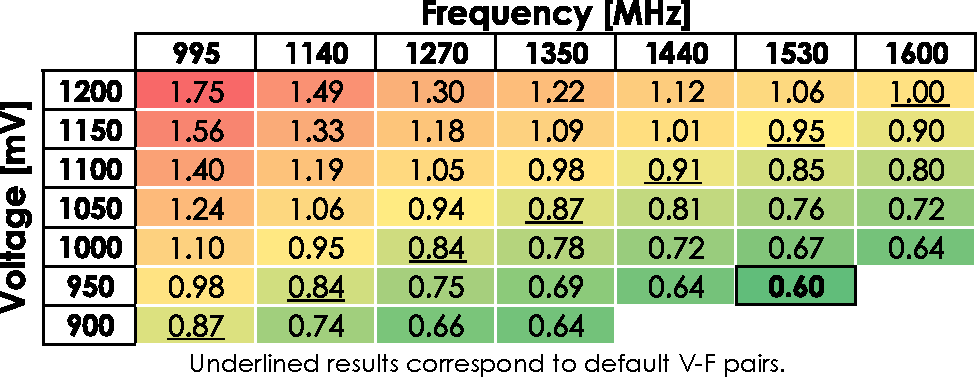
\includegraphics[width=0.53\textwidth]{Figures/GPU_characterization/CacheL2_EDP_OPS0.pdf}
        \label{fig:Vega10-cache_edp}
      }
      \subfigure[Radeon 5700 XT.]{
        \centering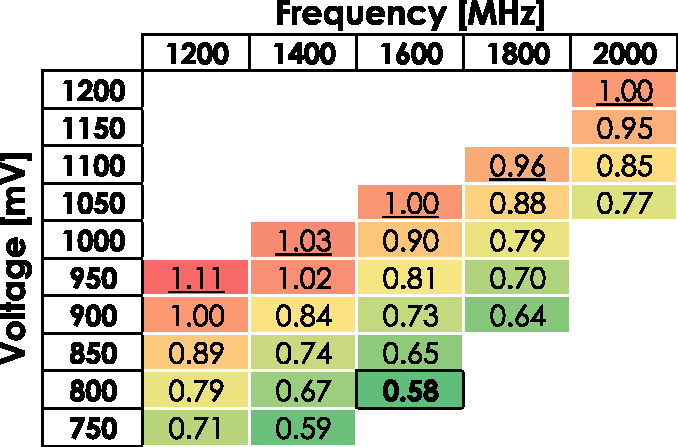
\includegraphics[width=0.37\textwidth]{Figures/GPU_characterization/5700XT-CacheL2_EDP_OPS0.pdf}
        \label{fig:5700XT-cache_edp}
      }
    \end{subfigmatrix}
    \caption{Core domain - Cache L2 - Obtained normalized Energy-Delay Product (EDP) with \texttt{OPS}=0.}
\end{figure}

% \begin{figure}[!htb]
%   \begin{subfigmatrix}{2}
%     \subfigure[Cache]{\label{fig:cacheL2_behaviour}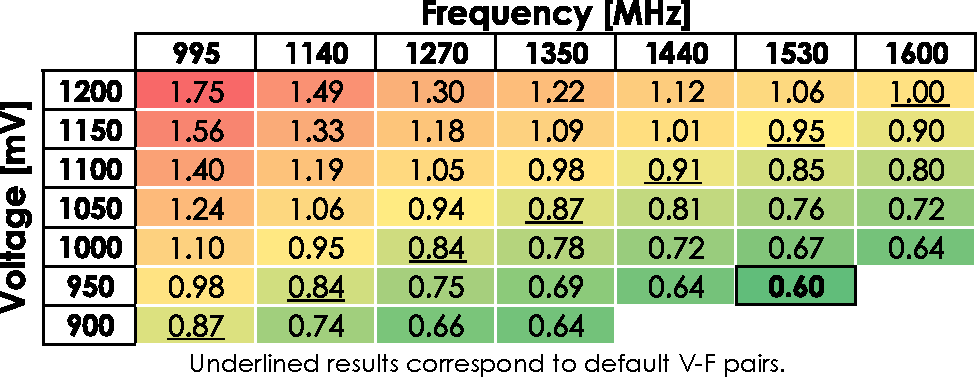
\includegraphics[width=0.47\textwidth]{Figures/GPU_characterization/CacheL2_EDP_OPS0.pdf}}
%     \subfigure[Shared Memory]{\label{fig:sm_behaviour}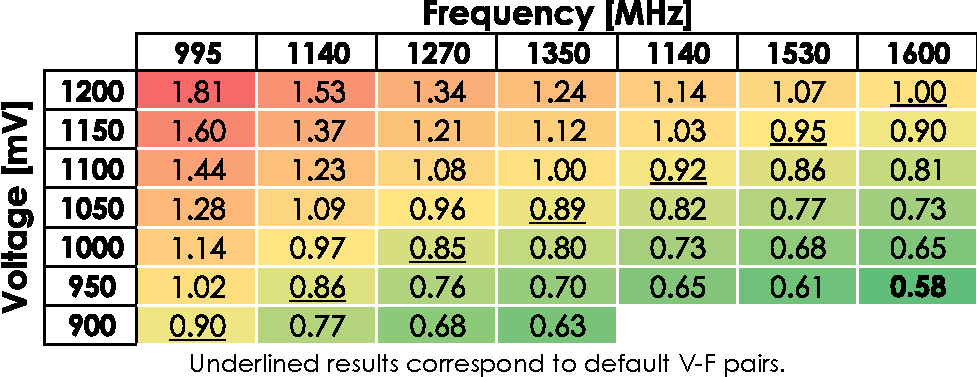
\includegraphics[width=0.47\textwidth]{Figures/GPU_characterization/SM_EDP_OPS0.pdf}}
%   \end{subfigmatrix}
%   \caption{Core domain - Obtained Energy-Delay Product (EDP) for \texttt{OPS}=0.}
%   \label{fig:cache_sm_edp}
% \end{figure}

% \begin{figure}[htb]
%   \centering
%   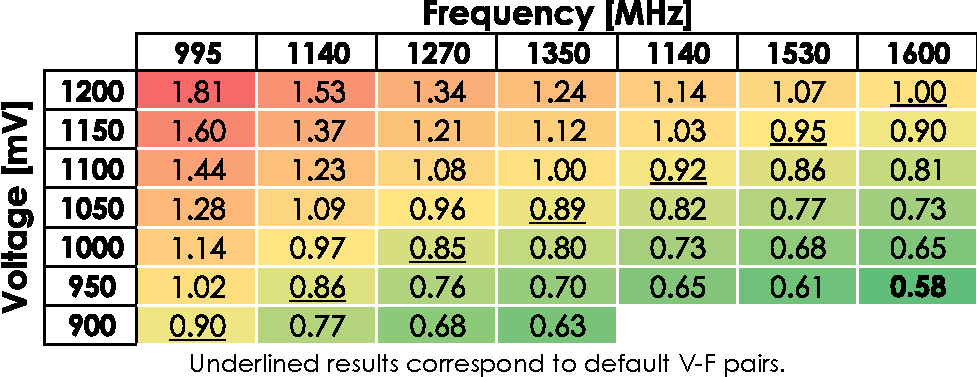
\includegraphics[width=0.5\textwidth]{Figures/GPU_characterization/SM_EDP_OPS0.pdf}
%   \caption{Vega 10 - Core domain - Shared Memory - Obtained Energy-Delay Product (EDP) with \texttt{OPS}=0.}
%   \label{fig:sm_edp}
% \end{figure}

\begin{figure}[!htb]
    \centering
    \begin{subfigmatrix}{2}
      \label{fig:sm_behaviour}
      \subfigure[Vega 10.]{
        \centering
        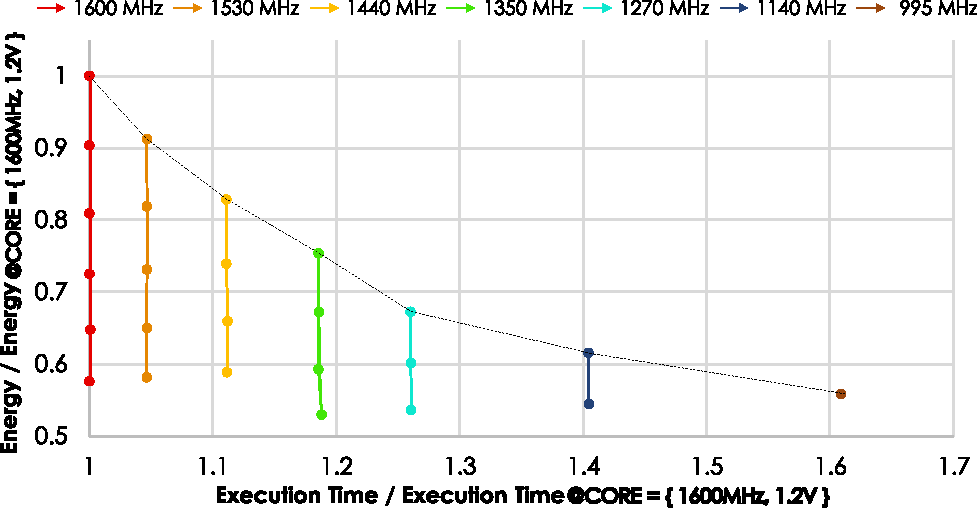
\includegraphics[width=0.45\textwidth]{Figures/GPU_characterization/SharedMemory_behaviour.pdf}
        \label{fig:Vega10-sm_behaviour}
      }
      \subfigure[Radeon 5700 XT.]{
        \centering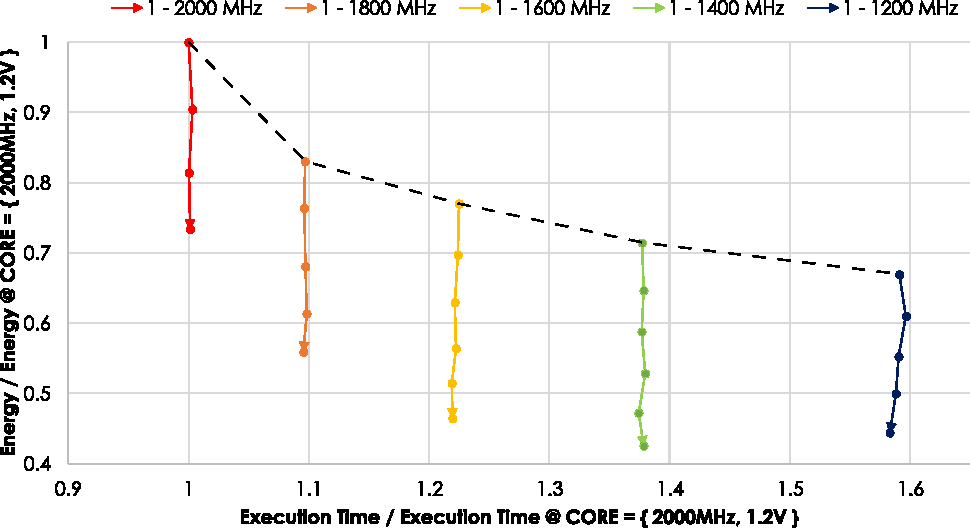
\includegraphics[width=0.45\textwidth]{Figures/GPU_characterization/5700XT-SharedMemory_Behaviour_0OP.pdf}
        \label{fig:5700XT-sm_behaviour}
      }
    \end{subfigmatrix}
    \caption{Core domain - Shared Memory - Normalized energy consumption and execution time. The dashed line connects the default F-V configurations and each connected data point represents a $50mV$ undervoltage in relation to the previous one.}
\end{figure}

\begin{figure}[!htb]
    \centering
    \begin{subfigmatrix}{2}
      \label{fig:sm_edp}
      \subfigure[Vega 10.]{
        \centering
        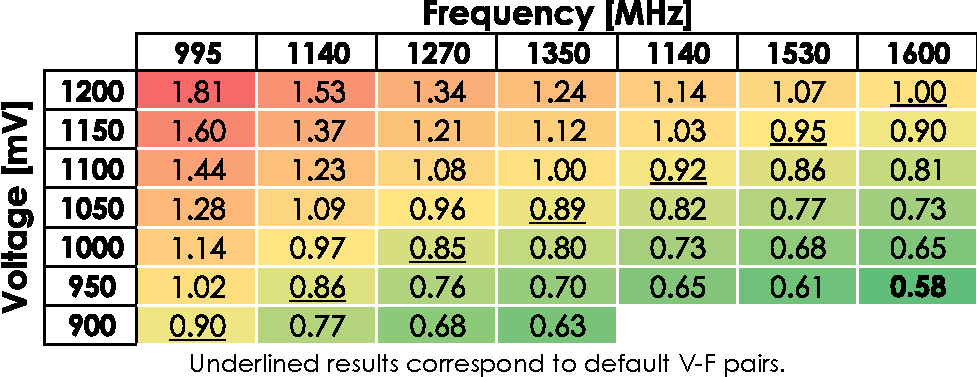
\includegraphics[width=0.5\textwidth]{Figures/GPU_characterization/SM_EDP_OPS0.pdf}
        \label{fig:Vega10-sm_edp}
      }
      \subfigure[Radeon 5700 XT.]{
        \centering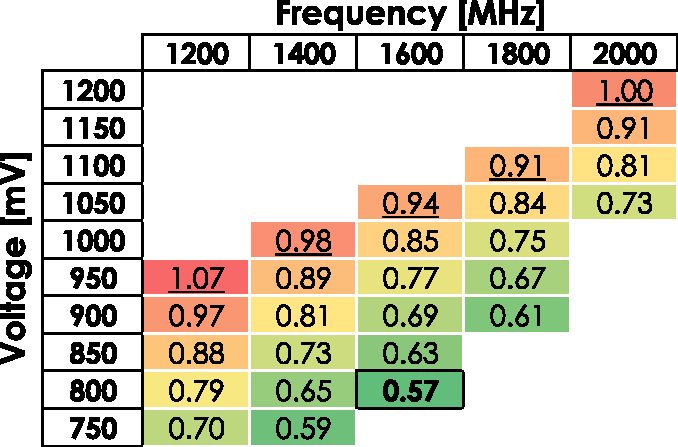
\includegraphics[width=0.35\textwidth]{Figures/GPU_characterization/5700XT-SharedMemory_EDP_0OP.pdf}
        \label{fig:5700XT-sm_edp}
      }
    \end{subfigmatrix}
    \caption{Core domain - Shared Memory - Obtained normalized Energy-Delay Product (EDP) with \texttt{OPS}=0.}
\end{figure}



\subsection{Arithmetic and Logic Unit}

\label{sec:MAC_behaviour}
Figure~\ref{fig:MAC_behaviour} represents the normalized (to the highest core domain V-F configuration) energy consumption and execution time of the \acrshort{mac} benchmark for different V-F pairs. In the figures that follow, it was chosen to represent the result of the single-precision floating-point data-type, since it is the most used. However, the results for the remaining data types are similar.

An interesting phenomenon is observed in the energy-execution time plot for the highest frequencies of both \acrshort{gpu}s. Performing undervoltage not only reduces energy consumption (as expected), but it also allows for faster execution time. An explanation can be found by analyzing the power consumption during the benchmark execution. For the default voltage, the power surpasses the power cap, which activates the GPU protection mechanisms, halting the execution until the power is reduced. By applying an undervoltage, the power significantly decreases (as $P_{Static}\propto V$ and $P_{Dynamic}\propto V^2$, see \cite{guerreiro_gpgpu_2018}) and allows a sustained maintenance of the desire DVFS configuration. 

% \begin{figure}[htb]
%   \centering
%   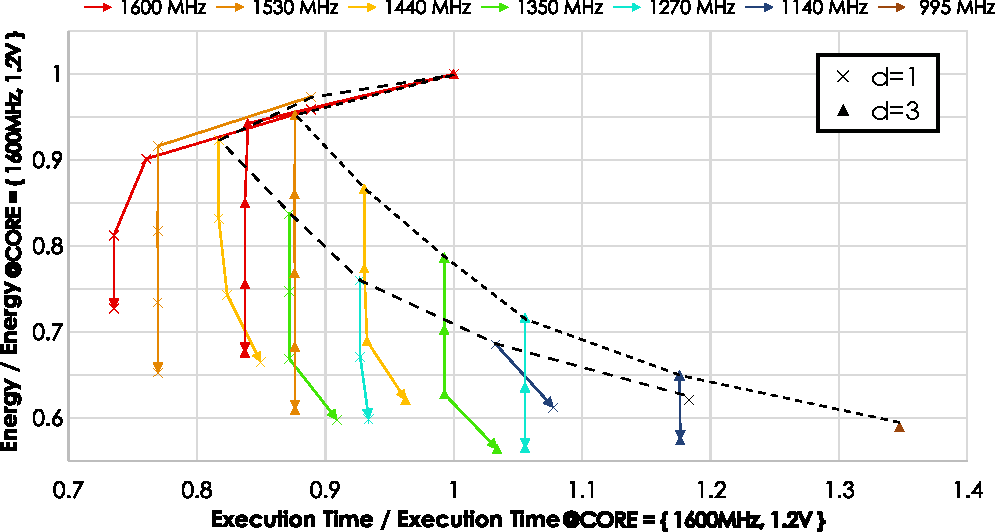
\includegraphics[width=0.8\textwidth]{Figures/GPU_characterization/MAC_behaviour_d_1_3.pdf}
%   \caption{Vega 10 - Core domain - ALU-MAC - Normalized energy and performance chart for the benchmark setup with different values of \texttt{d} for single precision floating-point (see Listing~\ref{lst:MACbench}). The dashed lines connect the results for default F-V configurations.}
%   \label{fig:MAC_behaviour}
% \end{figure}

\begin{figure}[!htb]
    \centering
    \begin{subfigmatrix}{2}
      \label{fig:MAC_behaviour}
      \subfigure[Vega 10.]{
        \centering
        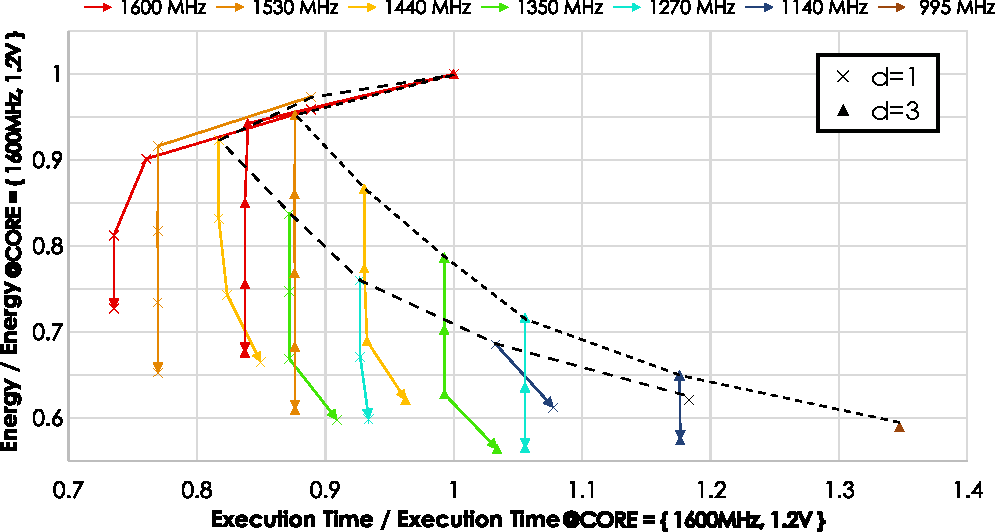
\includegraphics[width=0.45\textwidth]{Figures/GPU_characterization/MAC_behaviour_d_1_3.pdf}
        \label{fig:Vega10-MAC_behaviour}
      }
      \subfigure[Radeon 5700 XT.]{
        \centering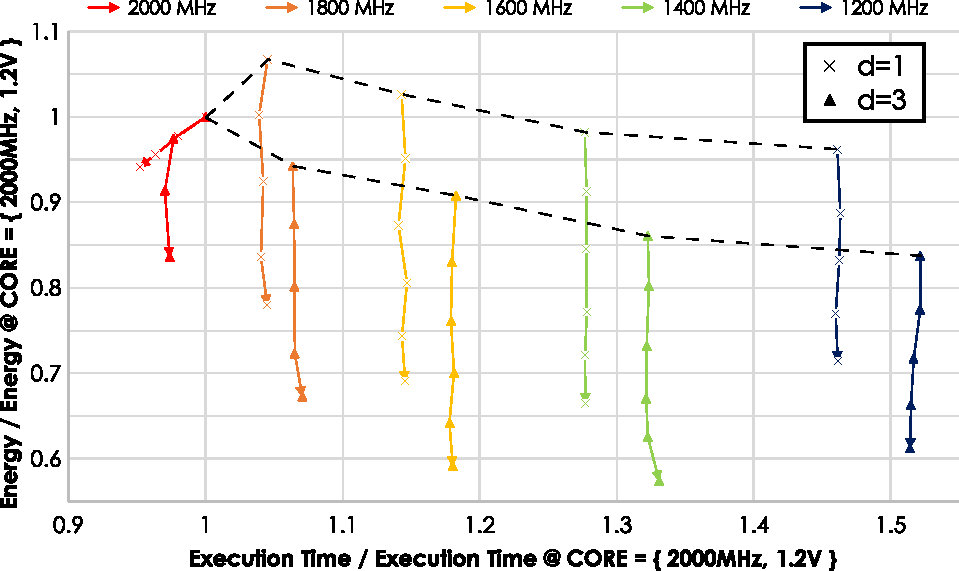
\includegraphics[width=0.45\textwidth]{Figures/GPU_characterization/5700XT-MAC_behaviour_d_1_3_sp.pdf}
        \label{fig:5700XT-MAC_behaviour}
      }
    \end{subfigmatrix}
    \caption{Core domain - ALU-MAC - Normalized energy and performance chart for the benchmark setup with different values of \texttt{d} for single precision floating-point (see Listing~\ref{lst:MACbench}). The dashed lines connect the results for default F-V configurations.}
\end{figure}

Finally, Figure~\ref{fig:MAC_EDP} presents the obtained EDP chart for single-precision floating-point data-type. The Vega 10 \acrshort{gpu} favors higher frequencies to achieve the best energy efficiency, while the Radeon 5700 XT achieves better results at the frequencies where it is possible to undervolt the most.

% \begin{figure}[htb]
%     \centering
%         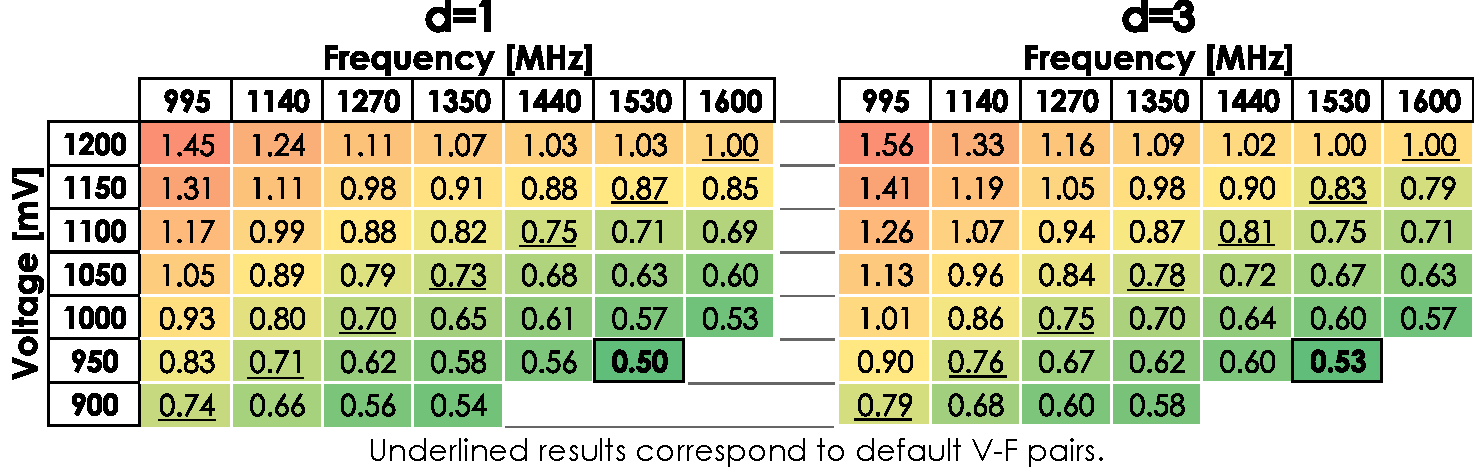
\includegraphics[width=0.8\textwidth]{Figures/GPU_characterization/MAC_EDP.pdf}
%         \caption{Core domain - ALU-MAC - Obtained Energy-Delay Product (EDP) for \texttt{d}=${1,3}$.}
%     \label{fig:MAC_EDP}
% \end{figure}

\begin{figure}[!htb]
    \centering
    \begin{subfigmatrix}{2}
      \label{fig:MAC_EDP}
      \subfigure[Vega 10.]{
        \centering
        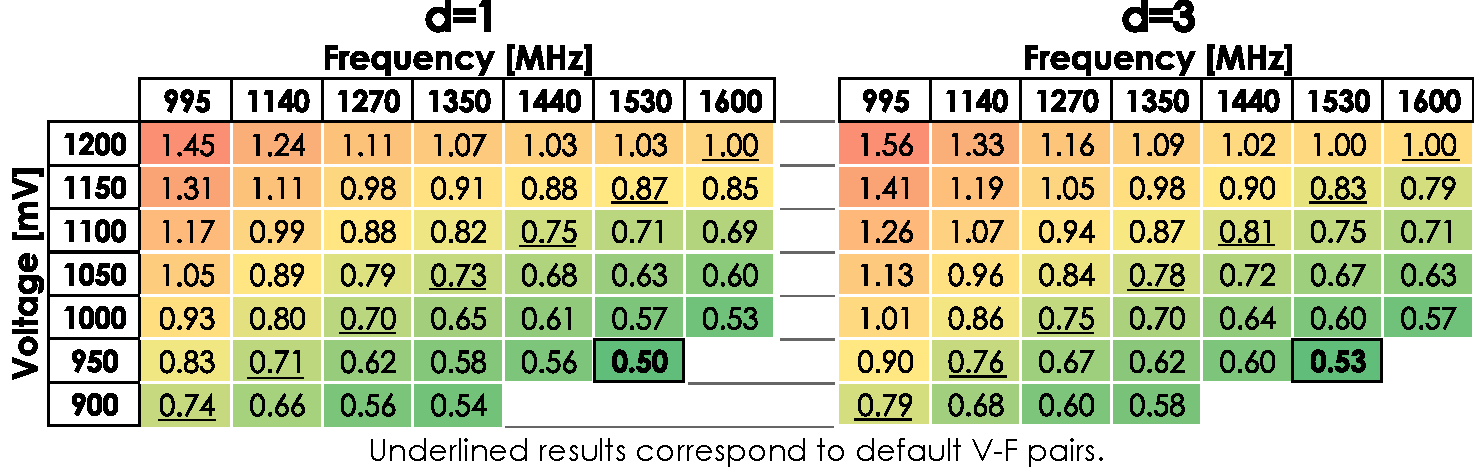
\includegraphics[width=0.8\textwidth]{Figures/GPU_characterization/MAC_EDP.pdf}
        \label{fig:Vega10-MAC_EDP}
      }
      \subfigure[Radeon 5700 XT.]{
        \centering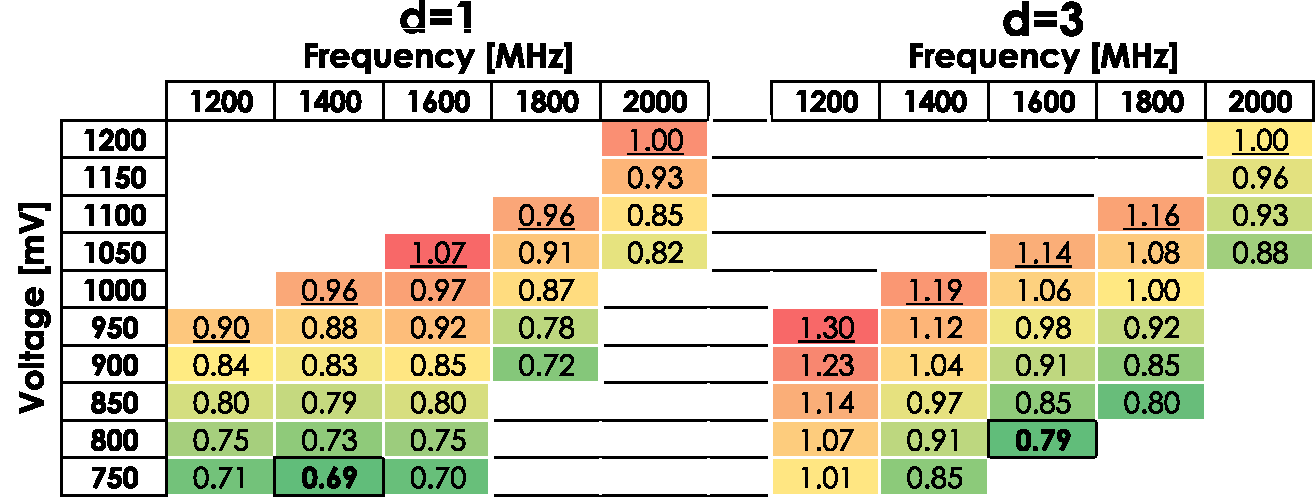
\includegraphics[width=0.7\textwidth]{Figures/GPU_characterization/5700XT-MAC_EDP.pdf}
        \label{fig:5700XT-MAC_EDP}
      }
    \end{subfigmatrix}
    \caption{Core domain - ALU-MAC - Obtained normalized Energy-Delay Product (EDP) for \texttt{d}=${1,3}$.}
\end{figure}

\subsection{Non-linear Operations}

Figure~\ref{fig:SFU_behaviour} showcases the normalized energy consumption and execution time for different V-F pairs for the single-precision floating-point \acrshort{sfu} benchmark. In this case, the \acrshort{gpu} behavior differs on the two architectures. Vega 10 displays a similar behavior, to Cache and Shared Memory benchmarks, with the applied undervoltage not affecting the  performance. On the other hand, the Radeon 5700 XT behavior to non-conventional V-F is more similar to the MAC benchmark. At the two highest frequencies, performing undervoltage has a more significant benefit on performance than on energy.

Overall, the degree of energy savings that is achieved goes in line with the previous results.



% \begin{figure}[htb]
%   \centering
%   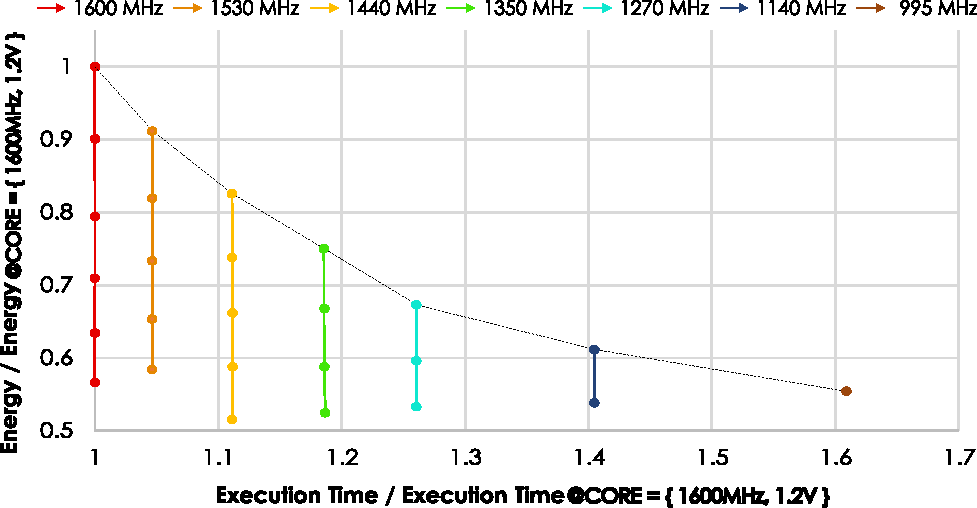
\includegraphics[width=0.7\textwidth]{Figures/GPU_characterization/SFU_behaviour.pdf}
%   \caption{Core domain - Special Function Unit - Normalized energy and performance for single-precision floating-point data type. The dashed lines connect the results for default F-V configurations.}
%   \label{fig:SFU_behaviour}
% \end{figure}

\begin{figure}[!htb]
    \centering
    \begin{subfigmatrix}{2}
      \label{fig:SFU_behaviour}
      \subfigure[Vega 10.]{
        \centering
        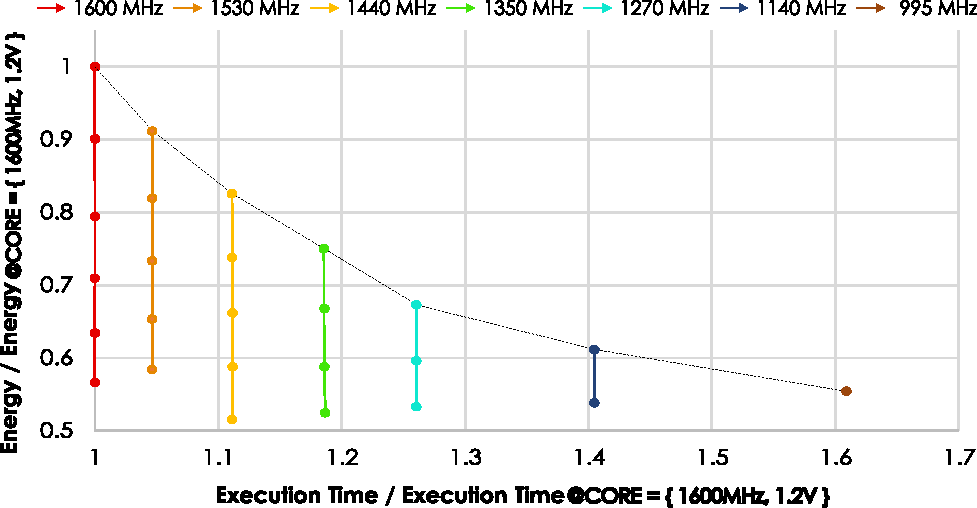
\includegraphics[width=0.45\textwidth]{Figures/GPU_characterization/SFU_behaviour.pdf}
        \label{fig:Vega10-SFU_behaviour}
      }
      \subfigure[Radeon 5700 XT.]{
        \centering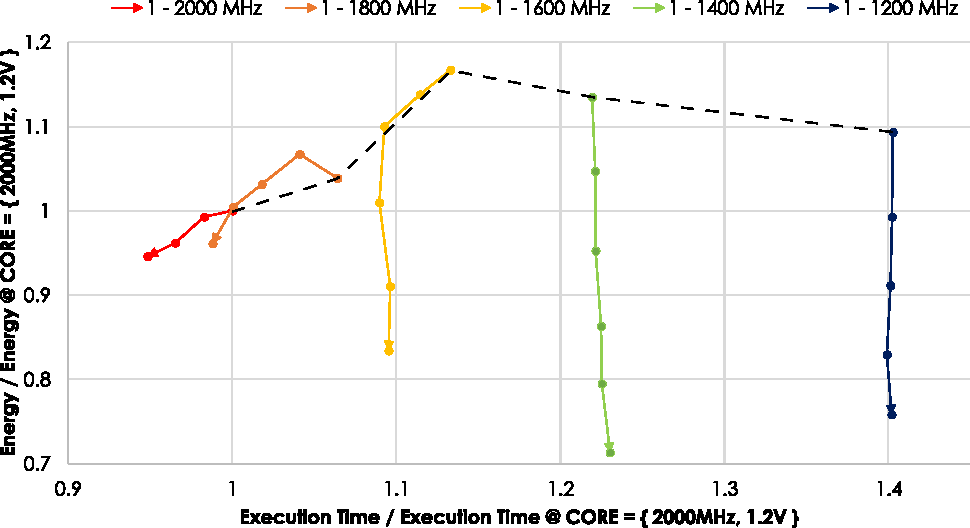
\includegraphics[width=0.45\textwidth]{Figures/GPU_characterization/5700XT-SFU_behaviour_sp.pdf}
        \label{fig:5700XT-SFU_behaviour}
      }
    \end{subfigmatrix}
    \caption{Core domain - Special Function Unit - Normalized energy and performance for single-precision floating-point data type. The dashed lines connect the results for default F-V configurations.}
\end{figure}

Figure~\ref{fig:SFU_EDP} represents the obtained  \acrshort{edp} heat-map, where it can be seen that the best energy efficiency is achieved with the highest amount of undervoltage, with this unit favoring lower frequencies on both \acrshort{gpu}s.

% \begin{figure}[htb]
%     \centering
%         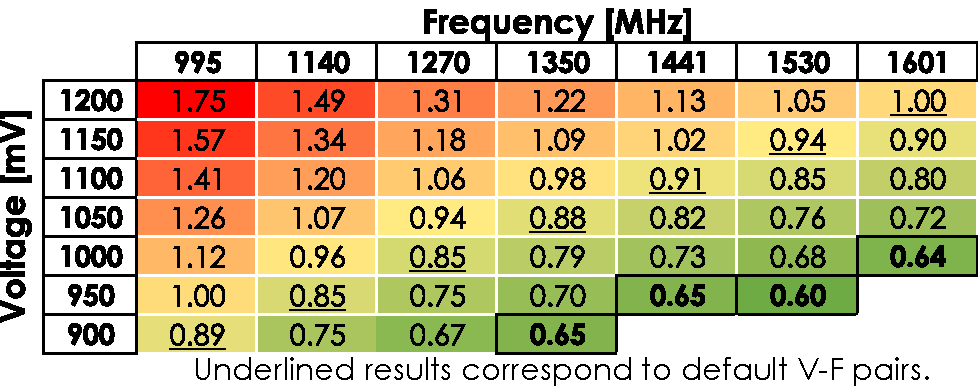
\includegraphics[width=0.55\textwidth]{Figures/GPU_characterization/SFU_EDP_SP.pdf}
%         \caption{Core domain - Special Function Unit - Obtained Energy-Delay Product (EDP) for single-precision floating-point data type.}
%     \label{fig:SFU_EDP}
% \end{figure}

\begin{figure}[!htb]
    \centering
    \begin{subfigmatrix}{2}
      \label{fig:SFU_EDP}
      \subfigure[Vega 10.]{
        \centering
        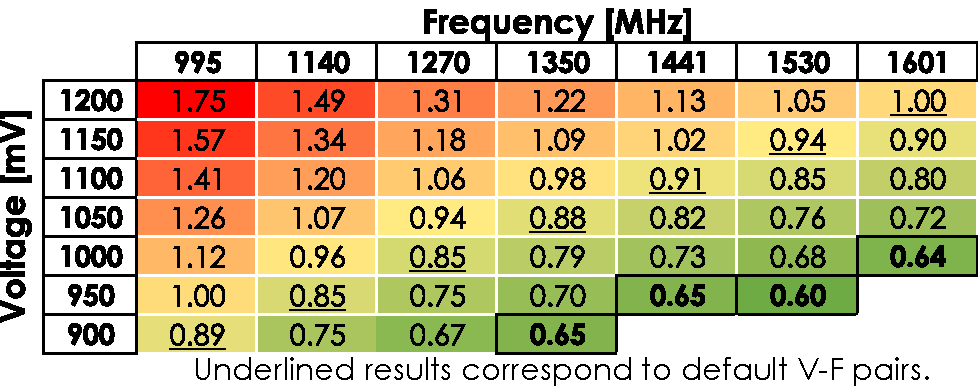
\includegraphics[width=0.53\textwidth]{Figures/GPU_characterization/SFU_EDP_SP.pdf}
        \label{fig:Vega10-SFU_EDP}
      }
      \subfigure[Radeon 5700 XT.]{
        \centering\includegraphics[width=0.37\textwidth]{Figures/GPU_characterization/5700XT-SFU_EDP_sp.pdf}
        \label{fig:5700XT-SFU_EDP}
      }
    \end{subfigmatrix}
    \caption{Core domain - Special Function Unit - Obtained Energy-Delay Product (EDP) for single-precision floating-point data type.}
\end{figure}


\section{Temperature Model}
\label{sec:temp_model}

The ALU and Cache L2 benchmarks were tested at a set temperature of 45ºC, by fixing the \acrshort{gpu} fan to 100\% and waiting for the temperature to stabilize between runs. This temperature was chosen by observing that the  \acrshort{gpu}'s temperature, while executing short benchmarks, stabilized around that temperature. However, during the execution of longer applications or when changing environmental conditions, the device can become hotter. The described work of Leng \textit{et al.}~\cite{leng_safe_2015} pointed out that only a small variation on $V_{min}$ is observed due to temperature variations. However, the performed experiments only cover temperatures up to 70ºC, easily surpassed by the \acrshort{gpu} underuse. 

To access the undervoltage capabilities in a broader range of temperatures, the benchmarks were continuously executed on both \acrshort{gpu}s, by varying the \acrshort{gpu} fan speed, and the output of the execution was analyzed. Varying the frequency did not change the temperature behavior, so the results of all executions were combined in Figure~\ref{fig:temp_model}, where only the results corresponding to voltage variations were represented. 

\begin{figure}[htb]
    \centering
        \includegraphics[width=0.7\textwidth]{Figures/GPU_characterization/UndervoltageWithTemperature_new.pdf}
        \caption{Undervoltage capabilties with changing temperature condition and defined temperature model.}
    \label{fig:temp_model}
\end{figure}

Hence, changing the amount of undervolt or fan speed resulted in the three different output scenarios. 
\textit{Working} - the benchmark's output was correct and was the same as when running with conventional V-F pairs.
\textit{Computation Errors} - the benchmark's output was not correct. However, the \acrshort{gpu} was still working and responding to the kernel commands. \textit{Crash} - the \acrshort{gpu} stop working and responding to the commands of the application.

Overall, the undervoltage capabilities stay relatively the same until the 70ºC to 75ºC temperature, with the highest undervoltage capabilities being achieved at the 55ºC mark. After the 75ºC mark, and following Freijado's work~\cite{freijedo_modeling_2012}, the carriers' mobility decreases and starts limiting the undervolting capabilities of the \acrshort{cmos} circuit. This result leads to the creation of a simple temperature model that limits the undervoltage potential for temperatures above 70ºC, as indicated in Figure~\ref{fig:temp_model}. This model acts as a fail-safe that guarantees that the non-conventional V-F exploration performed at 45ºC (as described until now) can be safely used across the complete temperature spectrum. The final user will have to limit the percentage of undervoltage according to this model, depending on the current \acrshort{gpu} temperature. By doing so, it guarantees that setting a safe non-conventional V-F pair will not cause a \acrshort{gpu} crash with temperature rise.




%%%%%%%%%%%%%%%%%%%%%%%%%%%%%%%%%%%%%%%%%%%%%%%%%%%%%%%%%%%%%%%%%%%%%%%%
\section{Summary}

The work presented in this chapter has three distinct objectives: 1) it acts as a feasibility assessment, allowing us to understand, measure and evaluate the degree of undervoltage that current \acrshort{gpu} architectures allow; 2) it characterizes the optimization space that one should consider to achieve the best energy-efficiency out of the devices; and 3), it works as a target energy-efficiency optimization benchmark to measure against non-conventional V-F pairs in complete applications.

After analyzing both \acrshort{dvfs} domains, the characterization of the Vega 10 \acrshort{gpu} showed that the \acrshort{dram} domain does not benefit from either non-conventional V-F pairs or even solely frequency scaling. AMD should have made the same conclusion since the next generation card (Radeon 5700 XT) omitted this \acrshort{dvfs} domain.

The following chapters will focus on improving the device energy efficiency by controlling the Core \acrshort{dvfs} domain. On this domain, it was found that both \acrshort{gpu}s significantly benefit from non-conventional V-F pairs, by allowing an increase of the energy efficiency at lower operating frequencies while having (and even surpassing) the performance corresponding to the traditional highest frequency and voltage configurations.
